\documentclass[a4paper]{article}

\setlength{\parindent}{0pt}
\setlength{\parskip}{1em}

\pagestyle{headings}

\usepackage{amssymb}
\usepackage{amsmath}
\usepackage{amsthm}
\usepackage{mathtools}
\usepackage{graphicx}
\usepackage{hyperref}
\usepackage{color}
\usepackage{microtype}
\usepackage{tikz}
\usepackage{pgfplots}
\usepackage{pgfplotstable}

\newcommand{\N}{\mathbb{N}}
\newcommand{\Q}{\mathbb{Q}}
\newcommand{\Z}{\mathbb{Z}}
\newcommand{\R}{\mathbb{R}}
\newcommand{\C}{\mathbb{C}}
\newcommand{\D}{\mathcal{D}}
\renewcommand{\S}{\mathcal{S}}
\renewcommand{\P}{\mathbb{P}}
\newcommand{\F}{\mathbb{F}}
\newcommand{\E}{\mathbb{E}}
\newcommand{\bra}{\langle}
\newcommand{\ket}{\rangle}


\graphicspath{{Image/}}

\hypersetup{
    colorlinks=true,
    linktoc=all,
    linkcolor=blue
}

\theoremstyle{definition}
\newtheorem*{axiom}{Axiom}
\newtheorem*{claim}{Claim}
\newtheorem*{conv}{Convention}
\newtheorem*{coro}{Corollary}
\newtheorem*{defi}{Definition}
\newtheorem*{eg}{Example}
\newtheorem*{lemma}{Lemma}
\newtheorem*{notation}{Notation}
\newtheorem*{prob}{Problem}
\newtheorem*{post}{Postulate}
\newtheorem*{prop}{Proposition}
\newtheorem*{rem}{Remark}
\newtheorem*{thm}{Theorem}

\DeclareMathOperator{\vdiv}{div}
\DeclareMathOperator{\grad}{grad}
\DeclareMathOperator{\curl}{curl}
\DeclareMathOperator{\Ann}{Ann}
\DeclareMathOperator{\Fit}{Fit}
\DeclareMathOperator{\Diag}{Diag}
\DeclareMathOperator{\tr}{tr}
\DeclareMathOperator{\im}{im}
\DeclareMathOperator{\Mat}{Mat}
\DeclareMathOperator{\Log}{Log}
\DeclareMathOperator{\Isom}{Isom}
\DeclareMathOperator{\Mesh}{Mesh}
\DeclareMathOperator{\Sym}{Sym}
\DeclareMathOperator{\Aut}{Aut}
\DeclareMathOperator{\cosech}{cosech}
\DeclareMathOperator{\Card}{Card}
\DeclareMathOperator{\Gal}{Gal}


\begin{document}

\title{Dynamics and Relativity}
\date{Lent 2016}

\maketitle

\newpage

\tableofcontents

\newpage

\section{System of masses}
\subsection{System of masses}
\subsubsection{Motion relative to the centre of mass}
Let $\mathbf{r_{i}}=\mathbf{R}+\mathbf{r_{i}}^c$, where $\mathbf{r_{i}}^c$ is the position of particle relative to the centre of mass.\\
Then\\
\begin{equation*}
\begin{aligned}
\sum_{i} m_{i}\mathbf{r_{i}}^c &= \sum_{i}m_{i} \mathbf{r_{i}}^c - \sum_{i} m_{i} \mathbf{R}\\
&=M\mathbf{R} - M\mathbf{R}\\
&=\mathbf{0}\\
& \implies \sum_{i}m_{i}\mathbf{\dot{r_{i}}}^c = \mathbf{0}.
\end{aligned}
\end{equation*}
The total linear momentum, angular momentum and kinetic energy are :\\
\begin{equation*}
\begin{aligned}
\mathbf{P} &= \sum_{i} m_{i}\left(\dot{\mathbf{R}}+\dot{\mathbf{r_{i}}}^c\right)\\
&= M\dot{\mathbf{R}}
\end{aligned}
\end{equation*}

\begin{equation*}
\begin{aligned}
\mathbf{L} &= \sum_{i} m_{i} \left(\mathbf{R}+ \mathbf{r_{i}}^c \right) \times \left(\dot{\mathbf{R}} + \dot{\mathbf{r_{i}}}^c\right)\\
&= \sum_{i} m_{i} \mathbf{R} \times \dot{\mathbf{R}} + \mathbf{R} \times \sum_{i} m_{i} \dot{\mathbf{r_{i}}}^c\\
&= M\mathbf{R}\times \dot{\mathbf{R}} + \sum_{i} m_{i} \mathbf{r_{i}}^c \times \dot{\mathbf{r_{i}}}^c.
\end{aligned}
\end{equation*}

\begin{equation*}
\begin{aligned}
T &= \frac{1}{2} \sum_{i} m_{i} |\dot{\mathbf{r_{i}}}|^2\\
&= \frac{1}{2} \sum_{i} m_{i} \left( \dot{\mathbf{R}} + \dot{\mathbf{r_{i}}}^c \right) \cdot \left( \dot{\mathbf{R}} + \dot{\mathbf{r_{i}}}^c \right)\\
&= \frac{1}{2} \sum_{i} m_{i} \dot{\mathbf{R}} \cdot \dot{\mathbf{R}} + \dot{\mathbf{R}}\cdot \sum_{i} m_{i}\dot{\mathbf{r_{i}}}^c + \frac{1}{2} \sum_{i} m_{i} \dot{\mathbf{r_{i}}}^c \cdot \dot{\mathbf{r_{i}}}^c\\
&= \frac{1}{2} M |\dot{\mathbf{R}}|^2 + \frac{1}{2} \sum_{i} m_{i} |\dot{\mathbf{r_{i}}}^c|^2\\
&= \text{KE of centre of mass + KE of motion relative to centre of mass.}
\end{aligned}
\end{equation*}

If the forces are conservative in the sense that 
\begin{equation*}
\begin{aligned}
\mathbf{F_{i}}^{ext} = -\nabla_{i} V_{i} \left(\mathbf{r_{i}}\right)
\end{aligned}
\end{equation*}
and $\mathbf{F_{ij}} = -\nabla_{i} V_{ij} \left(\mathbf{r_{i}}-\mathbf{r{j}}\right)$,\\
where $\nabla_{i}$ is the gradient with respect to $\mathbf{r_{i}}$, then energy is conserved in the form

\begin{equation*}
\begin{aligned}
E &= T + \sum_{i} V_{i} \left(\mathbf{r_{i}}\right) + \frac{1}{2} \sum_{i} \sum_{j} V_{ij}\left(\mathbf{r_{i}}-\mathbf{r_{j}}\right) &= constant.
\end{aligned}
\end{equation*}

\subsubsection{The two-body problem}
Consider two particles with no external forces.\\
The centre of mass is at \\
\begin{equation*}
\begin{aligned}
\mathbf{R} = \frac{1}{M}\left(m_{1}\mathbf{r_{1}}+m_{2}\mathbf{r_{2}}\right)
\end{aligned}
\end{equation*}
with $M=m_{1}+m_{2}$.\\
Define the separation vector(relative position vector):\\
\begin{equation*}
\begin{aligned}
\mathbf{r} = \mathbf{r_{1}}-\mathbf{r_{2}}.
\end{aligned}
\end{equation*}
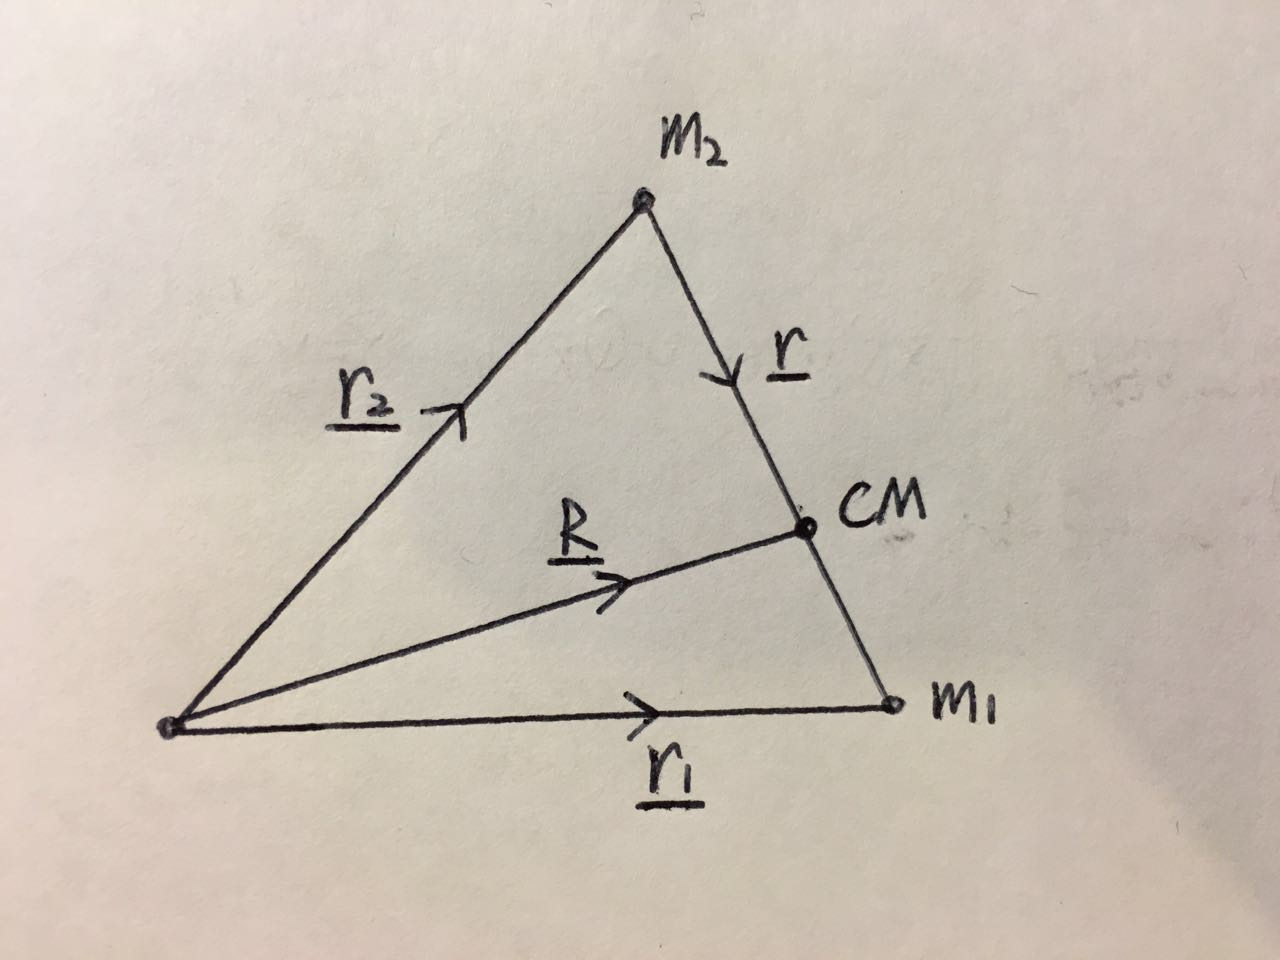
\includegraphics[scale=0.15]{Rel01}\\
Then 
\begin{equation*}
\begin{aligned}
\mathbf{r_{1}} = \mathbf{R} + \frac{m_{2}}{M}\mathbf{r},\\
\mathbf{r_{2}} = \mathbf{R} + \frac{m_{1}}{M}\mathbf{r}.
\end{aligned}
\end{equation*}

Since $\mathbf{F}=\mathbf{0}$ (no external forces), $\ddot{\mathbf{R}} = \mathbf{0}$.\\
The centre of mass moves uniformly.\\
Meanwhile,
\begin{equation*}
\begin{aligned}
\ddot{\mathbf{r}} &= \ddot{\mathbf{r_{1}}} - \ddot{\mathbf{r_{2}}}\\
&= \frac{1}{m_{1}} \mathbf{F_{12}} - \frac{1}{m_{2}} \mathbf{f_{21}}\\
&= \left(\frac{1}{m_{1}}+\frac{1}{m_{2}}\right)\mathbf{F_{12}} \text{ (using N3L)}
\end{aligned}
\end{equation*}

Thus
\begin{equation*}
\begin{aligned}
\mu \ddot{\mathbf{r}} &= \mathbf{F_{12}}\left(\mathbf{r}\right)
\end{aligned}
\end{equation*}
where 
\begin{equation*}
\begin{aligned}
\mu = \frac{m_{1}m_{2}}{m_{1}+m_{2}}
\end{aligned}
\end{equation*}
is the \emph{reduced mass}.\\
This is the same as the equation of motion for one particle of mass $\mu$ with position vector $\mathbf{r}$ relative to a fixed origin as studied previously.\\

\begin{eg} with gravity:
\begin{equation*}
\begin{aligned}
\mu \ddot{\mathbf{r}} &= -\frac{G m_{1} m_{2} \mathbf{r}}{|\mathbf{r}|^3} \implies \ddot{\mathbf{r}} = -\frac{GM\mathbf{\hat{r}}}{|\mathbf{r}|^2}
\end{aligned}
\end{equation*}
\end{eg}

\begin{eg} planet orbiting the Sun:\\
Both planet and Sun move in an ellipse about their centre of mass. Because the Sun is much more massive, its ellipse is much smaller. Orbital period depends on the total mass (Sun + planet).\\
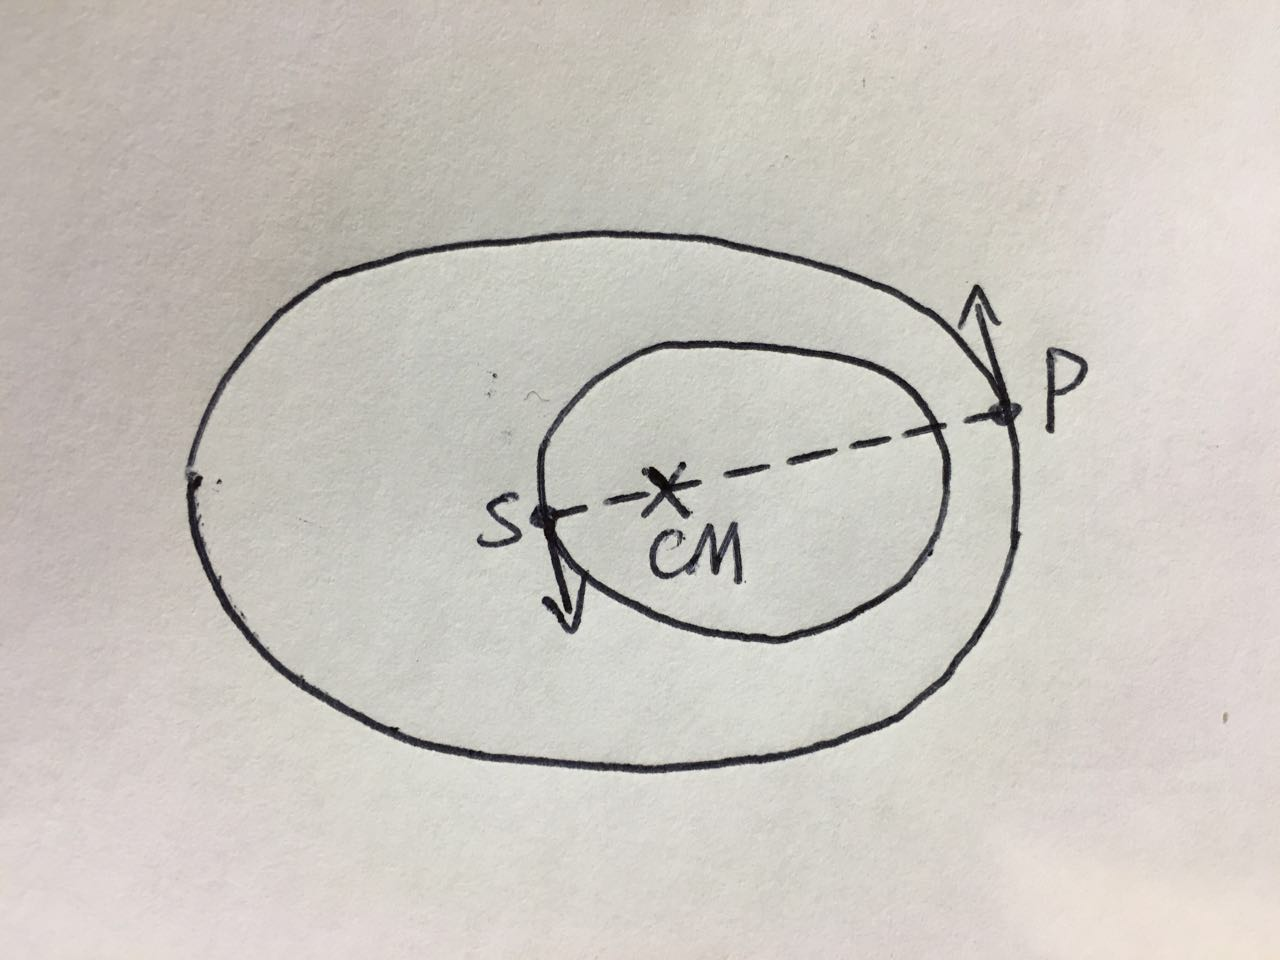
\includegraphics[scale=0.15]{Rel02}\\\\
Or binary black hole:\\
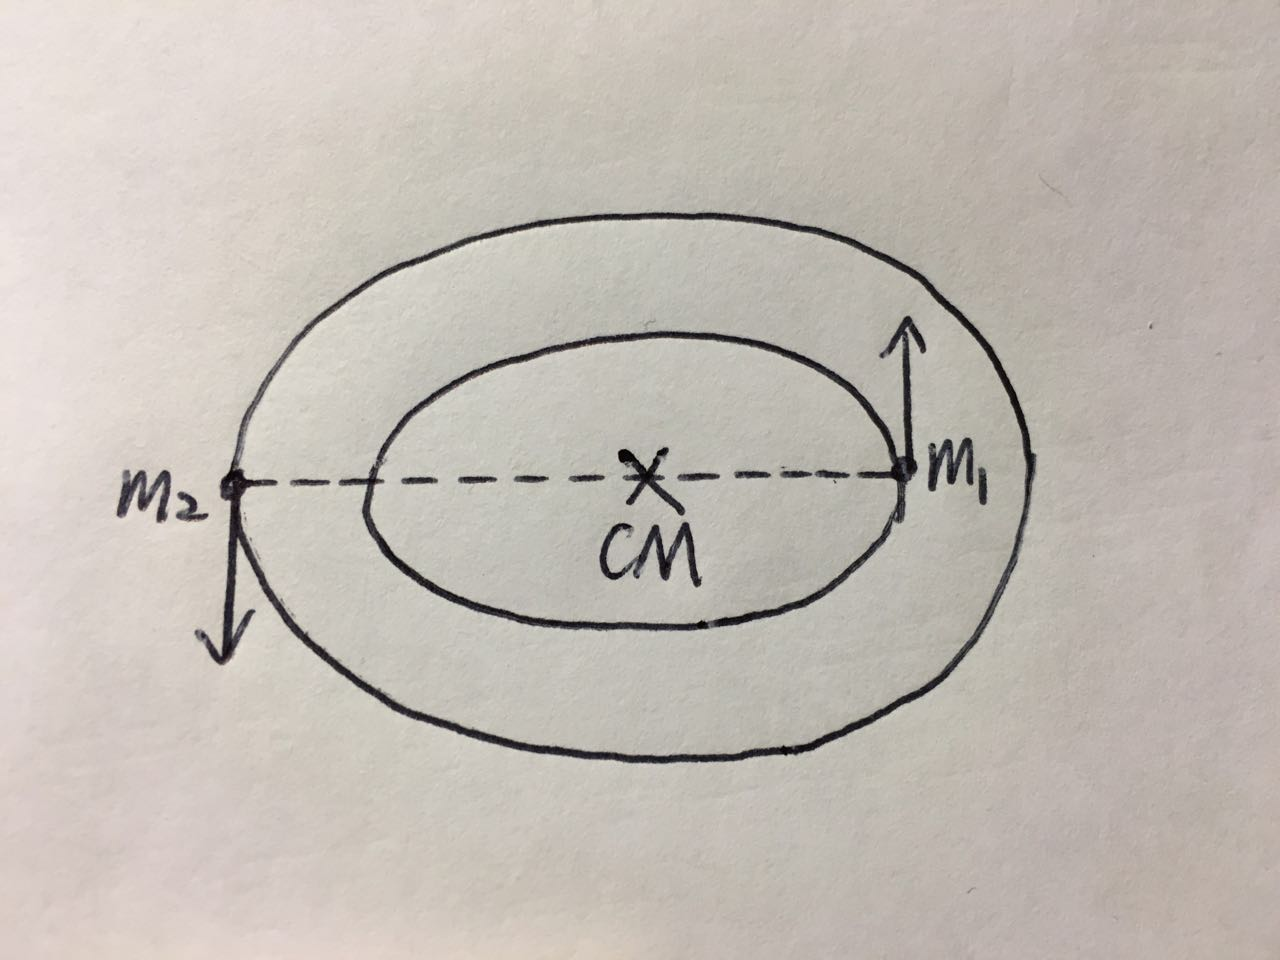
\includegraphics[scale=0.15]{Rel03}\\\\
It can be shown that
\begin{equation*}
\begin{aligned}
\mathbf{L} = M\mathbf{R}\times \dot{\mathbf{R}} + \mu \mathbf{r} \times \dot{\mathbf{r}}
\end{aligned}
\end{equation*}
\begin{equation*}
\begin{aligned}
T = \frac{1}{2} M |\dot{\mathbf{R}}|^2 + \frac{1}{2} \mu |\dot{\mathbf{r}}|^2
\end{aligned}
\end{equation*}
\end{eg}

\subsubsection{Variable-mass problems}
Newton's Second Law is\\
\begin{equation*}
\begin{aligned}
\dot{\mathbf{p}} = \mathbf{F} \text{ with } \mathbf{p} = m \dot{\mathbf{r}}
\end{aligned}
\end{equation*}
but we cannot simply apply this equation if $m$ depends on $t$ because that implies that the system is not closed.\\
Consider a rocket moving in one dimension, with mass $m\left(t\right)$ and velocity $v\left(t\right)$.\\
The rocket propels itself by burning fuel and ejecting the exhaust at velocity $-u$ relative to the rocket.\\
At time $t$:\\
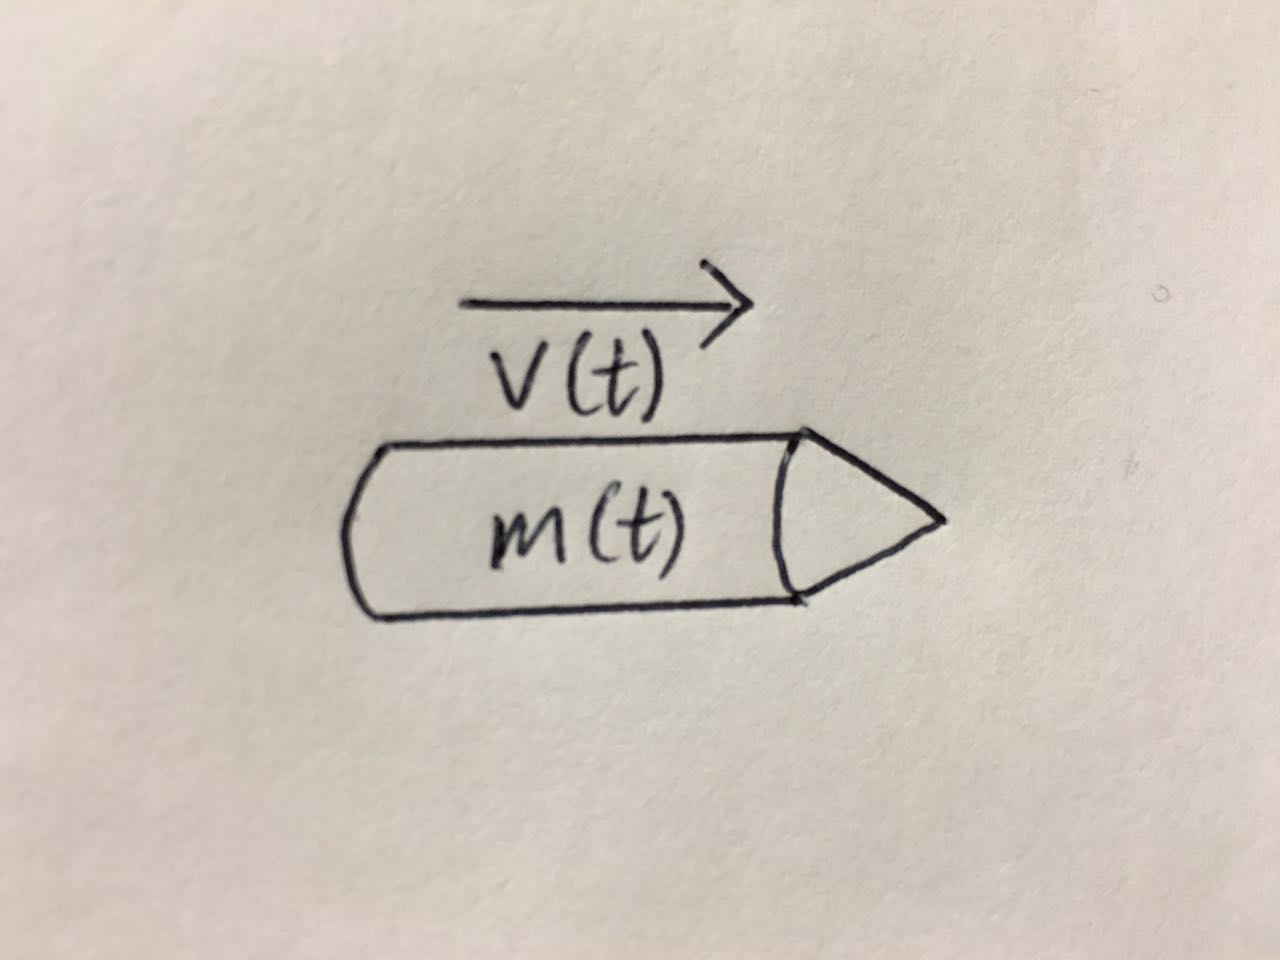
\includegraphics[scale=0.15]{Rel04}\\\\
At time $t+\delta t$:\\
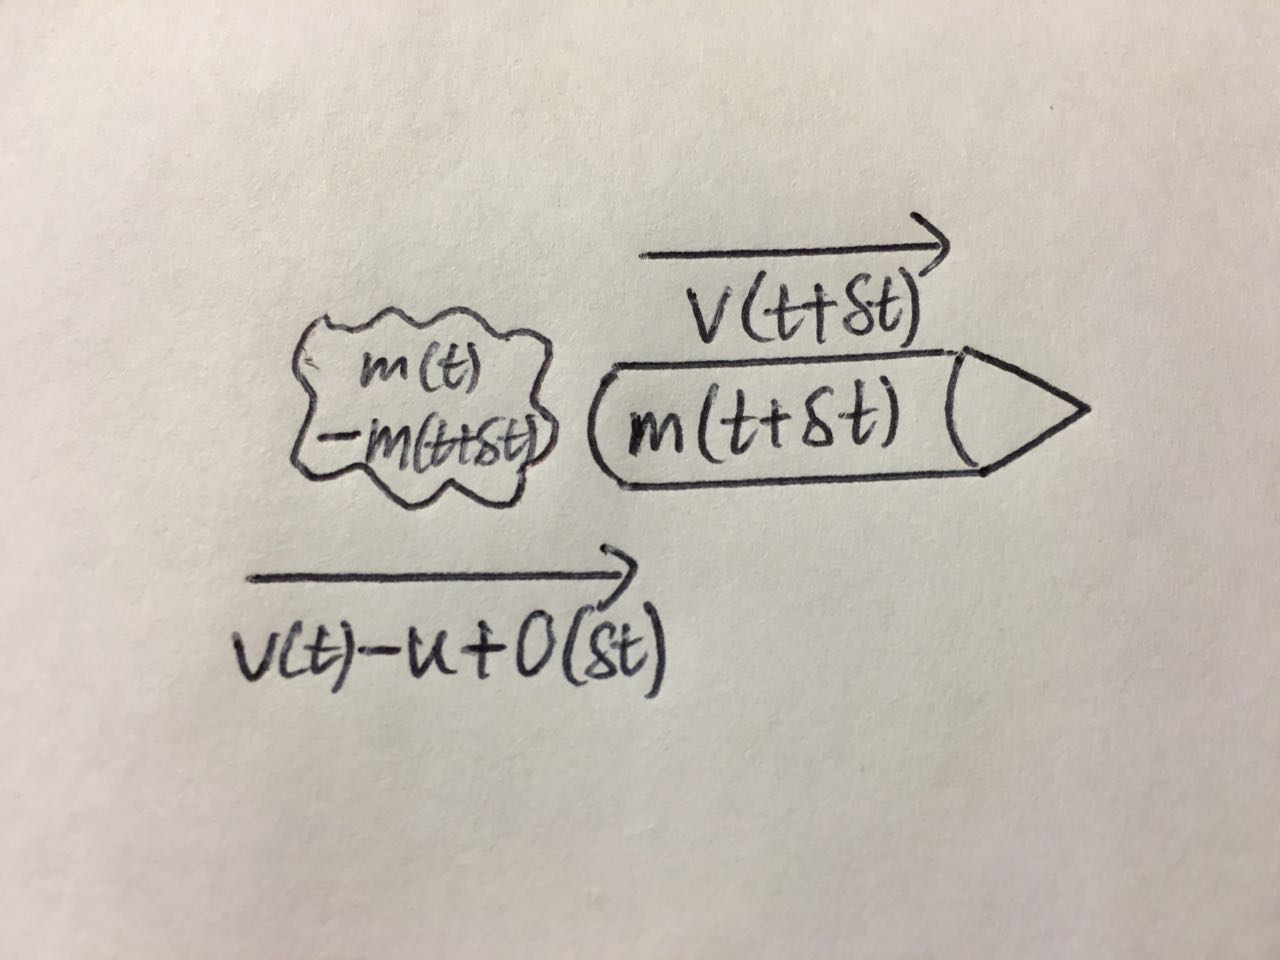
\includegraphics[scale=0.15]{Rel05}\\\\
The change in total momentum of the system (rocket+exhaust) is
\begin{equation*}
\begin{aligned}
\delta p &= m\left(t+\delta t\right) v\left(t+\delta t\right) + \left(m\left(t\right)-m\left(t+\delta t\right)\right)\left(v\left(t\right)-u+O\left(\delta t\right)\right)-m\left(t\right)v\left(t\right)\\
&=\left(m+\dot{m}\delta t+O\left(\delta t^2\right)\right)\left(v+\dot{v}\delta t+O\left(\delta t^2\right)\right) - \left(\dot{m} \delta t\right)\left(v-u\right) + O\left(\delta t^2\right) - mv\\
&=\left(\dot{m}v+m\dot{v}-\dot{m}v+\dot{m}u\right)\delta t + O\left(\delta t^2\right)\\
&=\left(m\dot{v}+\dot{m}u\right)\delta t + O\left(\delta t^2\right).
\end{aligned}
\end{equation*}

Newton's Second Law then gives
\begin{equation*}
\begin{aligned}
\lim_{\delta t\to 0} \frac{\partial p}{\partial t} &= F \text{ (external force acting on rocket)}\\
& \implies m\frac{dv}{dt} + u\frac{dm}{dt} = F
\end{aligned}
\end{equation*}
known as the \emph{rocket equation}.

\begin{eg}
where $F=0$, we have
\begin{equation*}
\begin{aligned}
m\frac{dv}{dt} &= -u\frac{dm}{dt}\\
& \implies v=v_{0} + u\log \left(\frac{m_{0}}{m\left(t\right)}\right)
\end{aligned}
\end{equation*}
(constant such that $v=v_{0}$ when $m=m_{0}$).\\

\end{eg}

\subsection{Rigid bodies}
A \emph{rigid body} is an extended object, consisting of $N$ particles that are constrained such that the distance $|\mathbf{r_i}-\mathbf{r_j}|$ between any two particles is fixed.\\
The possible motions of a rigid body are the continuous isometries of Euclidean space: \emph{translations} and \emph{rotations}.\\

\subsubsection{Angular velocity}
Consider a single particle moving in a circle of radius $s$ about the $z$ axis.\\
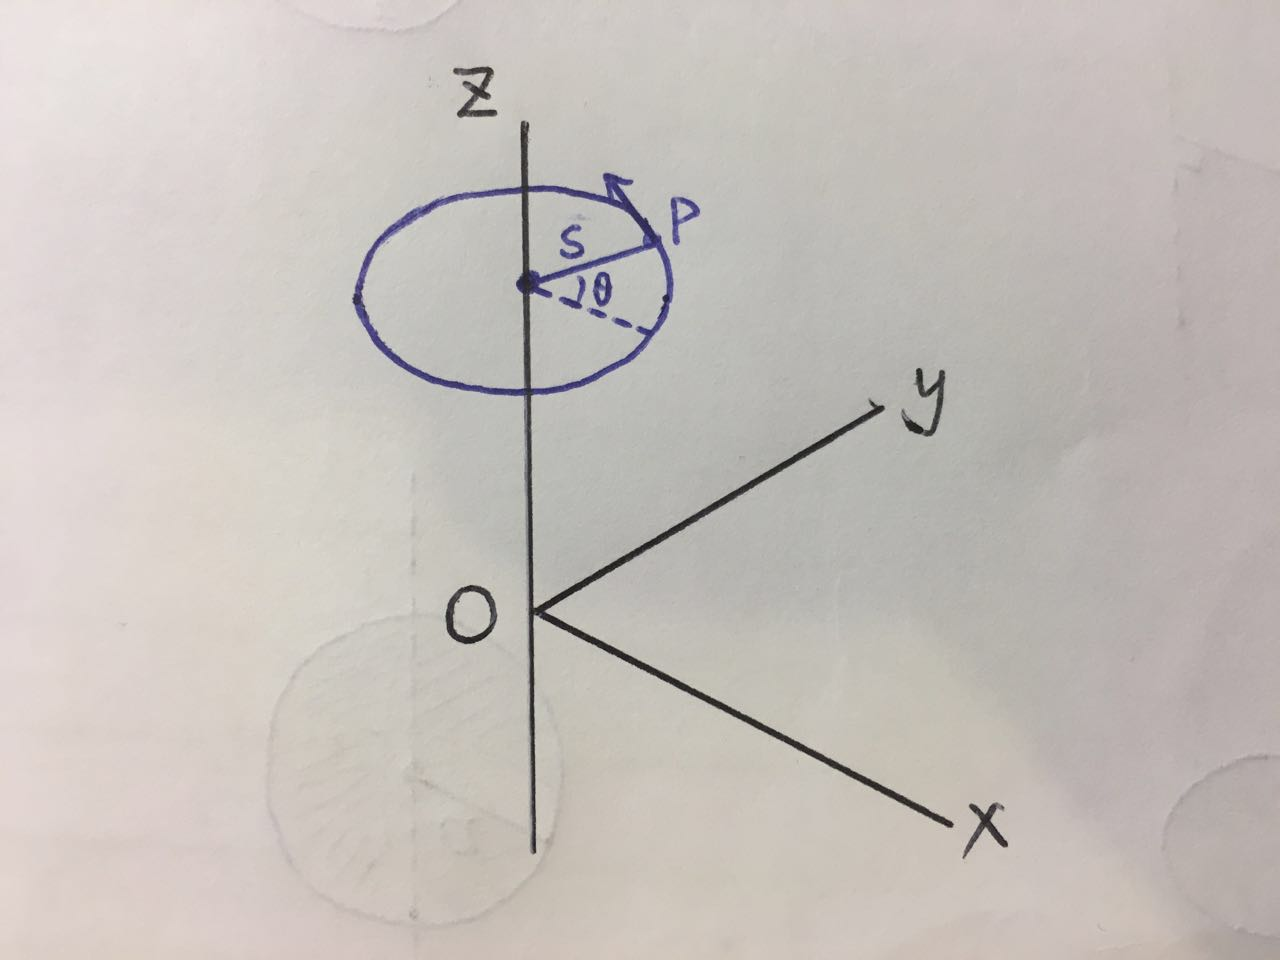
\includegraphics[scale=0.15]{Rel06}\\
Its position and velocity are\\
\begin{equation*}
\begin{aligned}
\mathbf{r}&=\left(s\cos \theta,s\sin\theta,z\right)\\
\mathbf{\dot{r}}\left(-s\dot{\theta}\sin\theta,s\dot{\theta}cos\theta,0\right)
\end{aligned}
\end{equation*}
Then $\mathbf{\dot{r}}=\mathbf{\omega}\times\mathbf{r}$,\\
where $\mathbf{\omega}=\dot{\theta}\hat{\mathbf{z}}$ is the angular velocity vector. In general, $\mathbf{\omega}=\dot{\theta}\hat{\mathbf{n}}=\omega \hat{\mathbf{n}}$ where $\hat{\mathbf{n}}$ is a unit vector parallel to rotation axis.\\
The kinetic energy of the particle is\\
$T=\frac{1}{2}m\left(\dot{\mathbf{r}}\right)^2=\frac{1}{2}ms^2\dot{\theta}^2=\frac{1}{2}I\omega ^2$\\
where $I=ms^2=m|\hat{\mathbf{n}}\times\mathbf{r}|^2$\\
is the \emph{moment of inertia}.

\subsubsection{Moment of inertia}
Consider a rigid body in which all $N$ particles rotate about the same axis with the same angular velocity:\\
$\dot{\mathbf{r_i}}=\mathbf{\omega}\times\mathbf{r_i}$\\.
This ensures that:
\begin{equation*}
\begin{aligned}
\frac{d}{dt}|\mathbf{r_i}-\mathbf{r_j}|^2 &= 2\left(\mathbf{\dot{r_i}}-\mathbf{\dot{r_j}}\right)\cdot\left(\mathbf{r_i}-\mathbf{r_j}\right)\\
&=2\left(\mathbf{\omega}\times\left(\mathbf{r_i}-\mathbf{r_j}\right)\right)\cdot\left(\mathbf{r_i}-\mathbf{r_j}\right)\\
&=0
\end{aligned}
\end{equation*}
as required for a rigid body.\\
The rotational kinetic energy is\\
\begin{equation*}
\begin{aligned}
T &= \frac{1}{2}\sum_{i=1}^N m_i |\dot{\mathbf{r_i}}|^2\\
&= \frac{1}{2}I\omega^2
\end{aligned}
\end{equation*}
where $I=\sum_{i=1}^N m_i s_i^2=\sum_{i=1}^N m_i |\hat{\mathbf{n}}\times\mathbf{r_i}|^2$\\
is the moment of inertia of the body about the rotation axis.\\
The angular momentum is
\begin{equation*}
\begin{aligned}
\mathbf{L}&=\sum_i m_i \mathbf{r_i}\times \dot{\mathbf{r_i}}\\
&= \sum_i m_i \mathbf{r_i}\times\left(\mathbf{\omega}\times\mathbf{r_i}\right)
\end{aligned}
\end{equation*}
with $\mathbf{\omega} = \omega \hat{\mathbf{n}}$, we have
\begin{equation*}
\begin{aligned}
\mathbf{L}\cdot\hat{\mathbf{n}}&=\omega \sum_i m_i \hat{\mathbf{n}}\cdot\left(\mathbf{r_i}\times\left(\hat{\mathbf{n}}\times\mathbf{r_i}\right)\right)\\
&= \omega \sum_i m_i \left(\hat{\mathbf{n}}\times\mathbf{r_i}\right)\cdot\left(\hat{\mathbf{n}}\times\mathbf{r_i}\right)\\
&= I\omega
\end{aligned}
\end{equation*}
In general, though, $\mathbf{L}$ may not be parallel to $\mathbf{\omega}$. We can write
\begin{equation*}
\begin{aligned}
\mathbf{L}&=\sum_i m_i \left(\left(\mathbf{r_i}\cdot\mathbf{r_i}\right)\mathbf{\omega}-\left(\mathbf{r_i}\cdot\mathbf{\omega}\right)\mathbf{r_i}\right)\\
&=\underline{\underline{I}}\mathbf{\omega}
\end{aligned}
\end{equation*}
where $\underline{\underline{I}}$ is the \emph{inertia tensor} represented by the symmetric matrix with components
\begin{equation*}
\begin{aligned}
I_{jk}&= \sum_i m_i\left(|\mathbf{r_i}|^2\delta_{jk}-\left(\mathbf{r_i}\right)_j\left(\mathbf{r_i}\right)_k\right)
\end{aligned}
\end{equation*}
If the body rotates about a principal axis (one of the three orthogonal eigenvectors of $\underline{\underline{I}}$) e.g. on axis of symmetry if the body has one, then $\mathbf{L}$ is parallel to $\mathbf{\omega}$.\\
The relations $T=\frac{1}{2}I\omega^2$ and $L=I\omega$ for angular motion are analogous to the relations $T=\frac{1}{2}mv^2$ and $p=mv$ for linear motion.

\subsubsection{Calculating the moment of inertia}
For a solid body, we replace the sum over particle by a volume integral, weighted by the mass density $\rho\left(\mathbf{r}\right)$.\\
The mass
\begin{equation*}
\begin{aligned}
M=\int \rho dV,
\end{aligned}
\end{equation*}
the centre of mass is at
\begin{equation*}
\begin{aligned}
\mathbf{R}=\frac{1}{M}\int \rho\mathbf{r}dV
\end{aligned}
\end{equation*}
and the moment of inertia is
\begin{equation*}
\begin{aligned}
I=\int \rho s^2 dV=\int \rho |\hat{\mathbf{n}}\times\mathbf{r}|^2 dV
\end{aligned}
\end{equation*}
We mainly consider homogeneous bodies within which $\rho$ is a constant.\\
$\bullet$ Thin circular ring:\\
Mass $M$, radius $a$, rotation axis through centre, perpendicular to the plane of ring.\\
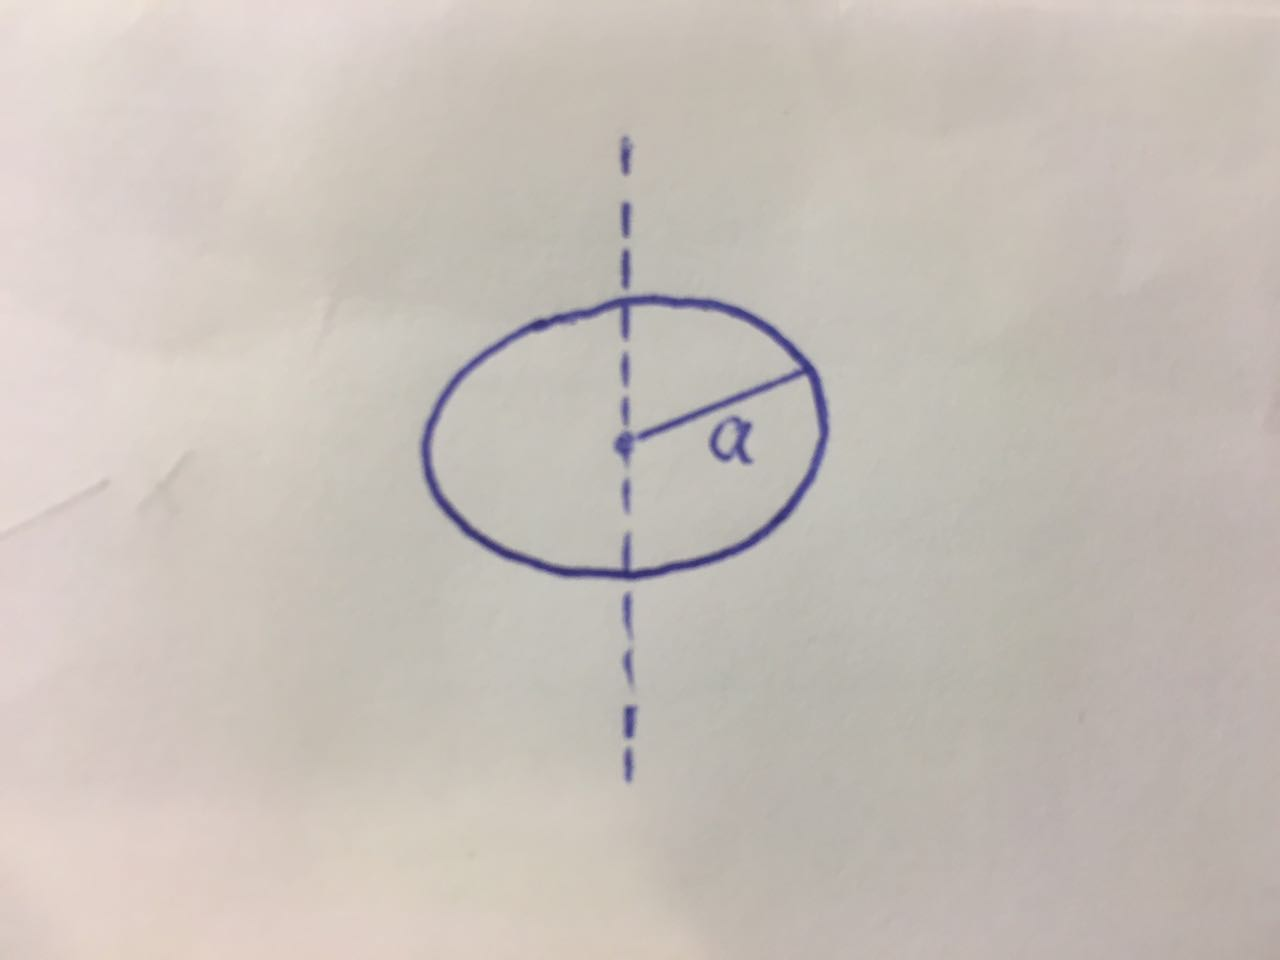
\includegraphics[scale=0.10]{Rel07}\\
$I=Ma^2$.\\

$\bullet$ Thin rod:\\
Mass $M$, length $l$, rotation axis through one end, perpendicular to the rod.\\
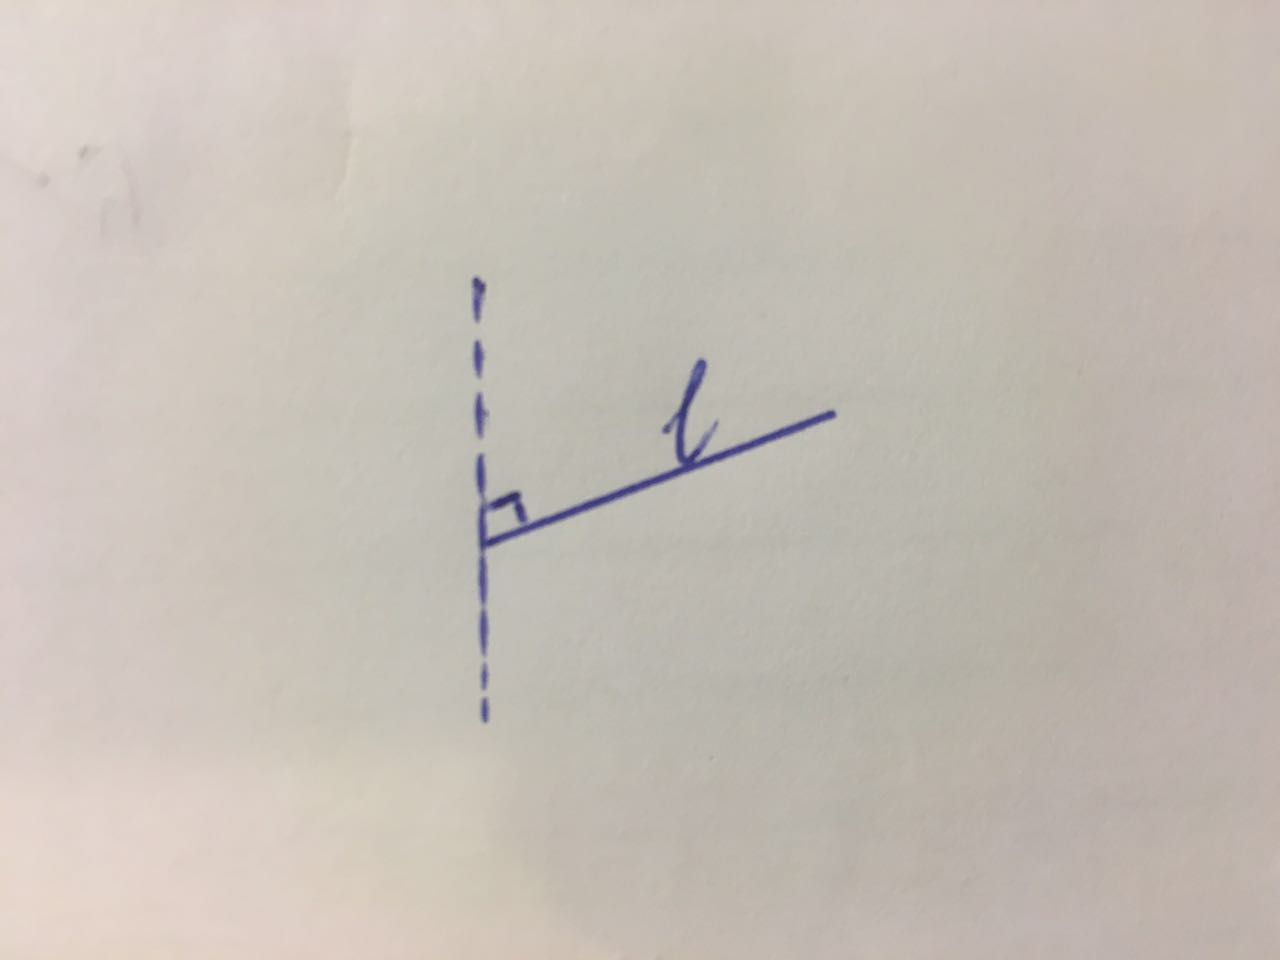
\includegraphics[scale=0.10]{Rel08}\\
\begin{equation*}
\begin{aligned}
I &= \int_0^l \frac{M}{l} x^2 dx\\
&= \frac{1}{3}Ml^2.
\end{aligned}
\end{equation*}

$\bullet$ Thin disc:\\
Mass $M$, radius $a$, rotation axis through center of disc perpendicular to the plane of disc:\\
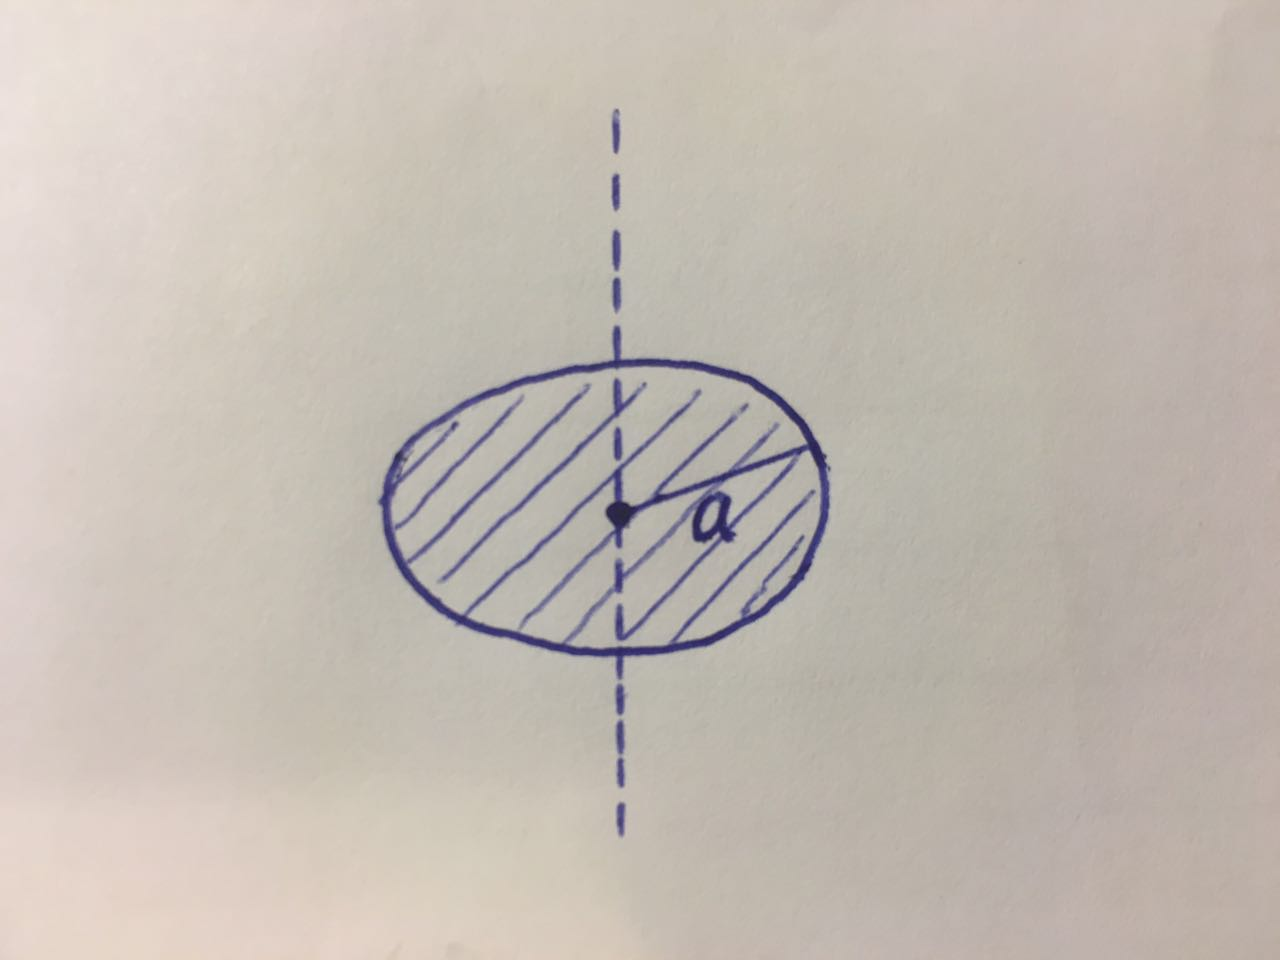
\includegraphics[scale=0.10]{Rel09}\\
\begin{equation*}
\begin{aligned}
I&=\int_0^{2\pi} \int_0^a \frac{M}{\pi a^2}r^2 rdrd\theta\\
&= \frac{M}{\pi a^2}\int_0^a r^3 dr \int_0^{2\pi} d\theta\\
&= \frac{M}{\pi a^2}\frac{1}{4}a^4\cdot 2\pi\\
&= \frac{1}{2}Ma^2.
\end{aligned}
\end{equation*}

Rotation axis through centre, in plane of disc:\\
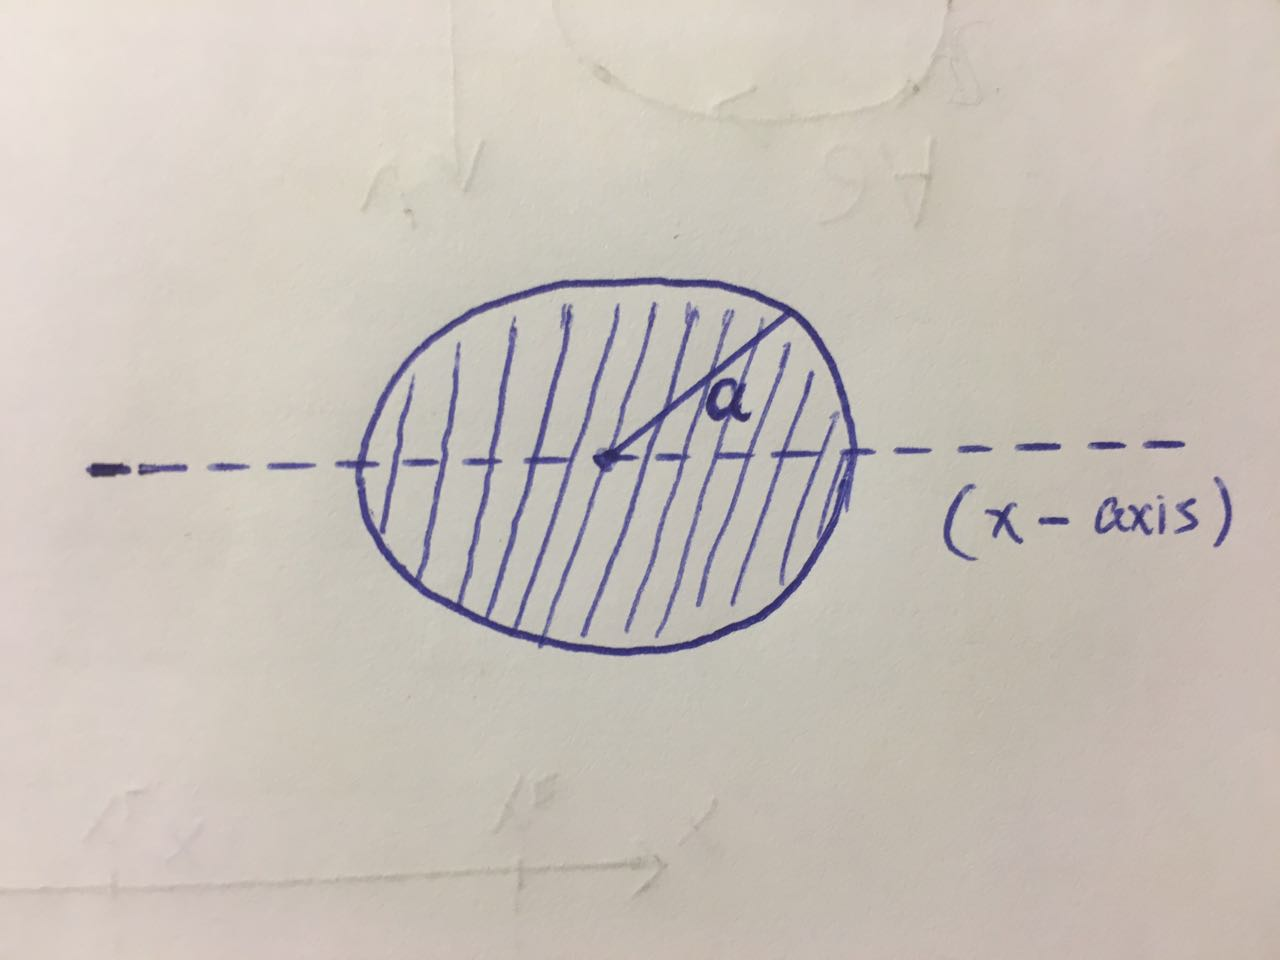
\includegraphics[scale=0.10]{Rel10}\\
\begin{equation*}
\begin{aligned}
I&=\int_0^{2\pi} \int_0^a \frac{M}{\pi a^2}\left(r\sin \theta\right)^2 rdrd\theta\\
&= \frac{M}{\pi a^2} \int_0^a r^2 dr \int_0^{2\pi} \sin^2 \theta d\theta\\
&= \frac{M}{\pi a^2}\frac{1}{4}a^4\cdot \pi\\
&=\frac{1}{4}Ma^2.
\end{aligned}
\end{equation*}

$\bullet$ Solid sphere:\\
Mass $M$, radius $a$, rotation axis through centre:\\
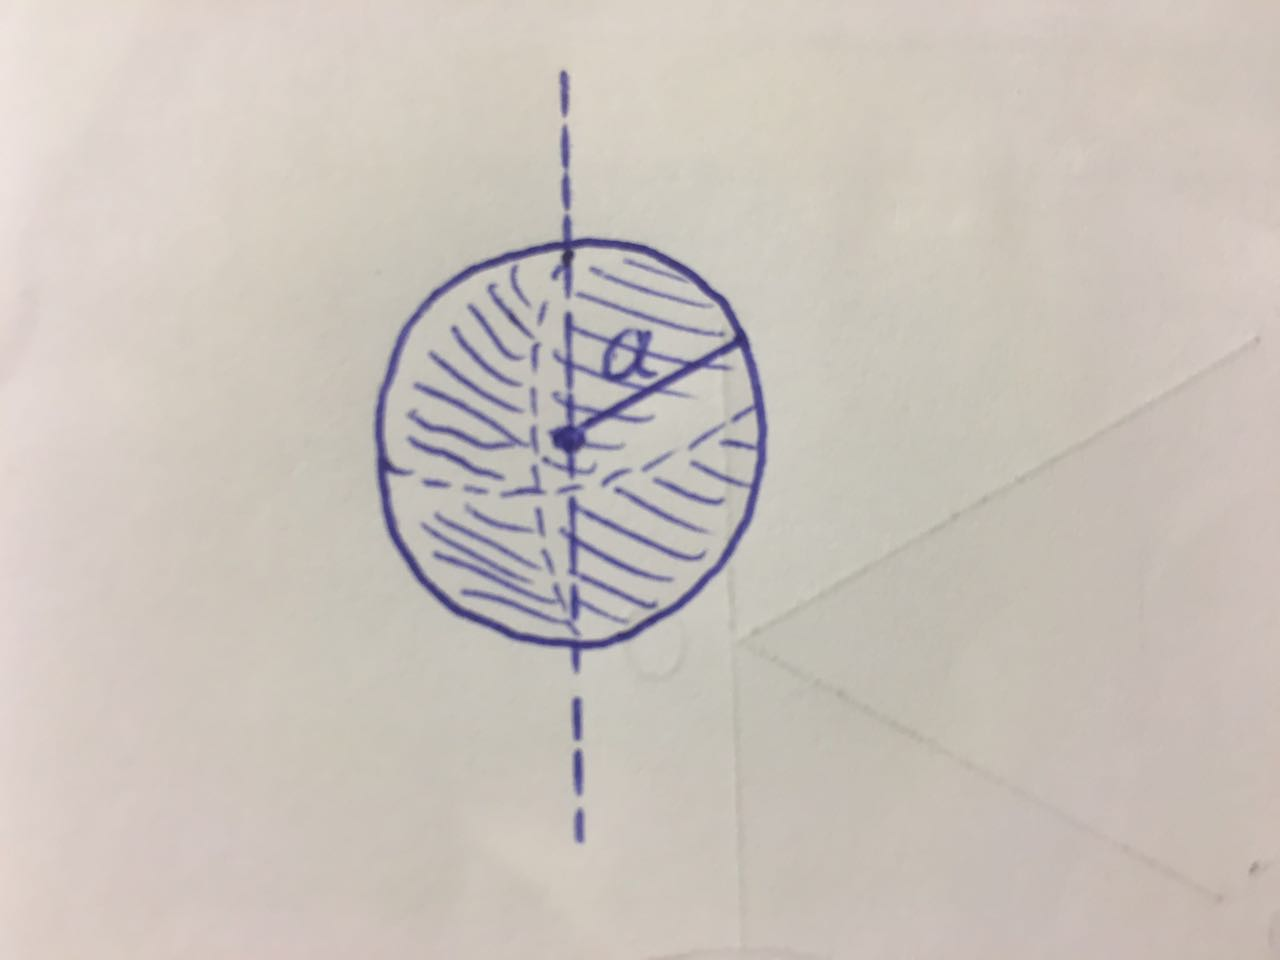
\includegraphics[scale=0.10]{Rel11}\\
Using spherical polar coordinates based on rotation axis:\\
\begin{equation*}
\begin{aligned}
I&= \int_0^{2\pi} \int_0^\pi \int_0^a \frac{M}{\frac{4}{3}\pi a^3}\left(r\sin\theta\right)^2 r^2 \sin\theta dr d\theta d\varphi\\
&=\frac{M}{\frac{4}{3}\pi a^3}\int_0^a r^4 dr \int_0^\pi \left(1-\cos^2\theta\right)\sin\theta d\theta \int_0^{2\pi} d\varphi\\
&=\frac{M}{\frac{4}{3}\pi a^3}\frac{1}{5}a^5\cdot \frac{4}{3}\cdot 2\pi\\
&=\frac{2}{5}Ma^2.
\end{aligned}
\end{equation*}

\begin{thm}(Perpendicular Axis Theorem)
For a two-dimensional object (a lamina) in the xy plane, and for three perpendicular axes through the same point,
\begin{equation*}
\begin{aligned}
I_z=I_x+I_y.
\end{aligned}
\end{equation*}
\begin{proof}
\begin{equation*}
\begin{aligned}
I_x &= \int \rho y^2 dA\\
I_y &= \int \rho x^2 dA\\
I_z &= \int \rho r^2 dA = \int \rho \left(x^2+y^2\right)dA=I_x + I_y.
\end{aligned}
\end{equation*}
\end{proof}
e.g. for a disc, $I_x = I_y$ by symmetry, so $I_z = 2I_x$.\\
Important: this does not apply to 3D objects (e.g. sphere, for which $I_x=I_y=I_z$).
\end{thm}

\begin{thm}(Parallel Axis Theorem)
If a rigid body of mass $M$ has moment of inertia $I^c$ about an axis passing through the centre of mass, then its moment of inertia about a parallel axis a distance $d$ away is $I=I^c + Md$.
\begin{proof}
With a convenient choice of Cartesian coordinates such that the centre of mass is at the origin and the two rotation axes are $x=y=0$ and $x=d, y=0$,
\begin{equation*}
\begin{aligned}
I^c &= \int \rho\left(x^2+y^2\right) dV
\end{aligned}
\end{equation*}
and
\begin{equation*}
\begin{aligned}
\int \rho\mathbf{r} dV = \mathbf{0}
\end{aligned}
\end{equation*}
Then
\begin{equation*}
\begin{aligned}
I &= \int \rho\left(\left(x-d\right)^2+y^2\right)dV\\
&= \int \rho\left(x^2+y^2\right)dV - 2d\int \rho x dV + d^2 \int \rho dV\\
&= I^c + Md^2.
\end{aligned}
\end{equation*}
\end{proof}
\end{thm}

\begin{eg}
Disc of mass $M$ and radius $a$:\\
rotation axis through point on circumference perpendicular to plane of the disc.
\begin{equation*}
\begin{aligned}
I&=I^c + Ma^2\\
&=\frac{1}{2}Ma^2 + Ma^2\\
&=\frac{3}{2}Ma^2
\end{aligned}
\end{equation*}
\end{eg}

\subsubsection{Motion of a rigid body}
The general motion of a rigid body can be described as a translation of its centre of mass, following a trajectory $\mathbf{R}\left(t\right)$, together with a rotation about an axis through the centre of mass.\\
We write
\begin{equation*}
\begin{aligned}
\mathbf{r_i} &= \mathbf{R}+\mathbf{r_i}^c\\
\implies \mathbf{\dot{r_i}} &= \mathbf{\dot{R}}+\mathbf{\dot{r_2}}^c
\end{aligned}
\end{equation*}
If the body rotates with angular velocity $\mathbf{w}$ about the centre of mass, then
\begin{equation*}
\begin{aligned}
\mathbf{\dot{r_i}}^c &= \mathbf{\omega} \times \mathbf{r_i}^c\\
\implies \mathbf{\dot{r_i}} &= \mathbf{\dot{R}} + \mathbf{\omega} \times\mathbf{r_i}^c\\
&=\mathbf{\dot{R}}+\mathbf{\omega}\times\left(\mathbf{r_i}-\mathbf{R}\right)
\end{aligned}
\end{equation*}
The kinetic energy is
\begin{equation*}
\begin{aligned}
T &= \frac{1}{2} M|\mathbf{\dot{R}}|^2 + \frac{1}{2}\sum_i m_i |\mathbf{\dot{r_i}}^c|^2\\
&= \frac{1}{2} M|\mathbf{\dot{R}}|^2 + \frac{1}{2}I^c \omega^2\\
&=\text{translational kinetic energy + rotational kinetic energy}
\end{aligned}
\end{equation*}
where $I^c$ is the moment of inertia about an axis parallel to $\mathbf{\omega}$ through the centre of mass.\\

Consider any point $Q$, with position vector $\mathbf{Q}\left(t\right)$, that is not the centre of mass but moves with the rigid body, i.e. 
\begin{equation*}
\begin{aligned}
\mathbf{\dot{Q}}&=\mathbf{\dot{R}}+\mathbf{\omega}\times\left(\mathbf{Q}-\mathbf{R}\right)
\end{aligned}
\end{equation*}
Then we can write
\begin{equation*}
\begin{aligned}
\mathbf{\dot{r_i}}&=\mathbf{\dot{R}}+\mathbf{\omega}\times\left(\mathbf{r_i}-\mathbf{R}\right)\\
&= \mathbf{\dot{Q}}-\mathbf{\omega}\times\left(\mathbf{Q}-\mathbf{R}\right)+\mathbf{\omega}\times\left(\mathbf{r_i}-\mathbf{R}\right)\\
&= \mathbf{\dot{Q}}+\mathbf{\omega}\times\left(\mathbf{r_i}-\mathbf{Q}\right).
\end{aligned}
\end{equation*}
Therefore the motion can be considered as a translation of the point (with a different velocity $\mathbf{\dot{Q}}\neq\mathbf{\dot{R}}$) together with a rotation about $Q$ (with the same angular velocity $\mathbf{\omega}$).\\

As shown previously, the linear and angular momentum evolve according to
\begin{equation*}
\begin{aligned}
\mathbf{\dot{P}}&=\mathbf{F} \text{  (total external force)}\\
\mathbf{\dot{L}}&=\mathbf{G} \text{  (total external torque)}
\end{aligned}
\end{equation*}
These two equations determine the translational and rotational motion of a rigid body. In some cases energy conservation is easier to apply.\\

$\mathbf{L}$ and $\mathbf{G}$ depend on the choice of origin, which could be any point that is fixed in an inertial frame, or the centre of mass, even if this is accelerated.
\begin{equation*}
\begin{aligned}
m\mathbf{\ddot{r_i}}=\mathbf{F_i} &\implies m_i \mathbf{\ddot{r_i}}^c = \mathbf{F_i}-\mathbf{m_i}\mathbf{\ddot{R}}
\end{aligned}
\end{equation*}
The last term is a fictitious force in the centre-of-mass frame. But the total torque of the fictitious forces about the centre of mass is
\begin{equation*}
\begin{aligned}
\sum_i \mathbf{r_i}^c \times \left(-m_i\mathbf{\ddot{R}}\right) &= -\sum_i m_i\mathbf{r_i}^c \times \mathbf{\ddot{R}} = \mathbf{0}.
\end{aligned}
\end{equation*}
In a uniform gravitational field $\mathbf{g}$, the total gravitational force and torque are the same as these would act on a single particle of mass $M$ located at the centre of mass (which is also the centre of gravity):
\begin{equation*}
\begin{aligned}
\mathbf{F}&= \sum_i \mathbf{F_i}^{ext} = \sum_i m_i \mathbf{g} = M\mathbf{g}\\
\mathbf{G}&= \sum_i \mathbf{G_i}^{ext} = \sum_i \mathbf{v_i}\times\left(m_i\mathbf{g}\right)=M\mathbf{R}\times\mathbf{g}.
\end{aligned}
\end{equation*}
Similarly for the gravitational potential energy, the gravitational potential in a uniform $\mathbf{g}$ is $-\mathbf{r}\cdot\mathbf{g}$(+ constant):
\begin{equation*}
\begin{aligned}
V^{ext} &= \sum_i V_i^{ext} = \sum_i m_i\left(-\mathbf{r}\cdot\mathbf{g}\right)=M\left(-\mathbf{R}\cdot\mathbf{g}\right)
\end{aligned}
\end{equation*}
In particular, the gravitational torque about the centre of mass vanishes:
\begin{equation*}
\begin{aligned}
\mathbf{G}^c = \mathbf{0}.
\end{aligned}
\end{equation*}

\begin{eg}
thrown stick:
The centre of the stick moves in a parabola.\\
Meanwhile, it rotates with constant angular velocity about its centre, because the gravitational torque about the centre is zero.
\end{eg}

\begin{eg} swinging rod:\\
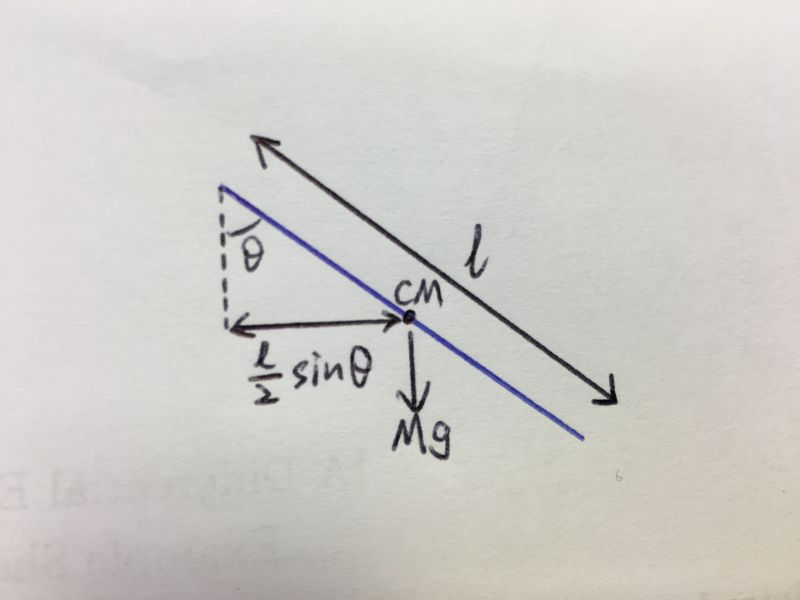
\includegraphics[scale=0.25]{Rel12}\\
This is an example of a compound pendulum.\\
Considering the rod to be rotating about the pivot (and not translating), its angular momentum is
\begin{equation*}
\begin{aligned}
L=I\dot{\theta}, I=\frac{1}{3}Ml^2
\end{aligned}
\end{equation*}
The gravitational torque about the pivot is
\begin{equation*}
\begin{aligned}
G=-Mg\frac{l}{2}\sin\theta
\end{aligned}
\end{equation*}
The equation of motion is
\begin{equation*}
\begin{aligned}
&\dot{L}=G\\
&\implies I\ddot{\theta}=-Mg\frac{l}{2}\sin\theta\\
&\implies \ddot{\theta}=-\frac{3g}{2l}\sin\theta
\end{aligned}
\end{equation*}
is exactly equivalent to a simple pendulum of length $\frac{2l}{3}$. The angular frequency of small oscillations is
\begin{equation*}
\begin{aligned}
\sqrt{\frac{3g}{2l}}.
\end{aligned}
\end{equation*}
Can also be obtained from an energy argument:
\begin{equation*}
\begin{aligned}
E=T+V = \frac{1}{2}I \dot{\theta}^2 - Mg\frac{l}{2}\cos\theta
\end{aligned}
\end{equation*}
Differentiate:
\begin{equation*}
\begin{aligned}
\frac{dE}{dt}&=\dot{\theta}\left(I\ddot{\theta}+Mg\frac{l}{2}\sin\theta\right) = 0\\
\implies I\ddot{\theta}&=-Mg\frac{l}{2}\sin\theta
\end{aligned}
\end{equation*}
\end{eg}

\subsubsection{Sliding versus rolling}
Consider a cylinder or sphere of radius $a$ moving along a stationary horizontal surface.\\
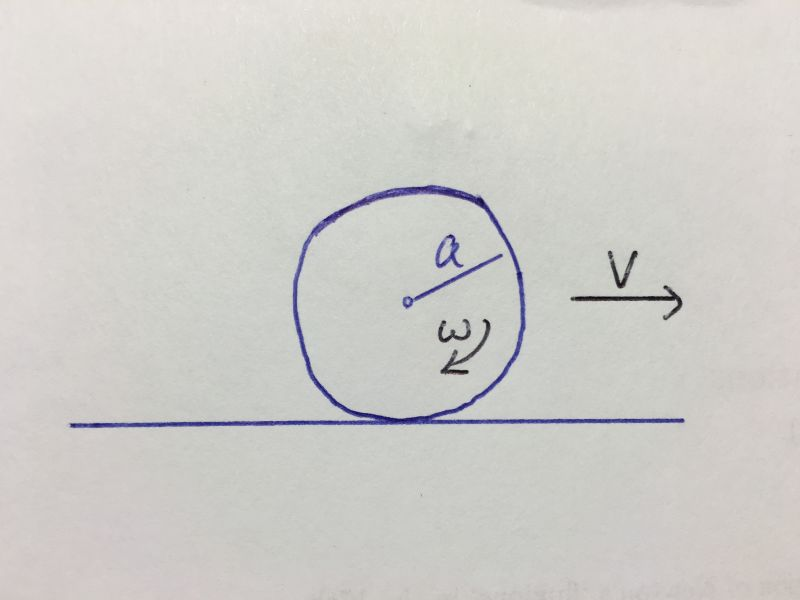
\includegraphics[scale=0.20]{Rel13}\\
In general, the motion consists of a translation of the centre of mass (with velocity $v$) together with a rotation about the centre of mass (with angular velocity $\omega$).\\
The horizontal velocty at the point of contact is 
\begin{equation*}
\begin{aligned}
v_{slip} = v-a\omega
\end{aligned}
\end{equation*}
For a pure sliding motion, $v\neq 0$ and $\omega =0$, in which case $v-a\omega \neq 0$: the point of contact slips on the surface and kinetic friction may occur.\\
Fora pure rolling motion, $v\neq 0$ and $w\neq 0$, such that $v-a\omega =0$. The point of contact is stationary (instantaneously). This is the \emph{no-slip condition}.\\
The rolling body can alternatively be considered to be rotating instantaneously about the point of contact (with angular velocity $\omega$) and not translating.

\begin{eg} (rolling downhill)\\
Cylinder or sphere of mass $M$ and radius $a$ rolling down a rough plane inclined at angle $\alpha$.\\
No-slip (rolling) condition: $v-a\omega = 0$.\\
Kinetic energy:
\begin{equation*}
\begin{aligned}
T&=\frac{1}{2}Mv^2+\frac{1}{2}I\omega^2\\
&=\frac{1}{2}\left(M+\frac{I}{a^2}\right)v^2
\end{aligned}
\end{equation*}
Total energy:
\begin{equation*}
\begin{aligned}
E&=\frac{1}{2}\left(M+\frac{I}{a^2}\right)\dot{x}^2-Mgx\sin\alpha
\end{aligned}
\end{equation*}
($x$ is distance down slope).
\end{eg}

Energy is conserved (see later):
\begin{equation*}
\begin{aligned}
&\frac{dE}{dt}=\dot{x}\left(\left(M+\frac{I}{a^2}\right)\ddot{x}-Mg\sin\alpha\right)=0\\
\implies &\left(M+\frac{I}{a^2}\right)\ddot{x}=Mg\sin\alpha.
\end{aligned}
\end{equation*}

\begin{eg} uniform solid cylinder:\\
\begin{equation*}
\begin{aligned}
&I=\frac{1}{2}Ma^2\\
\implies & \ddot{x}=\frac{2}{3}g\sin\alpha
\end{aligned}
\end{equation*}
For a hollow cylinder (thin cylindrical shell),
\begin{equation*}
\begin{aligned}
&I=Ma^2
\implies &\ddot{x}=\frac{1}{2}g\sin\alpha
\end{aligned}
\end{equation*}
\end{eg}
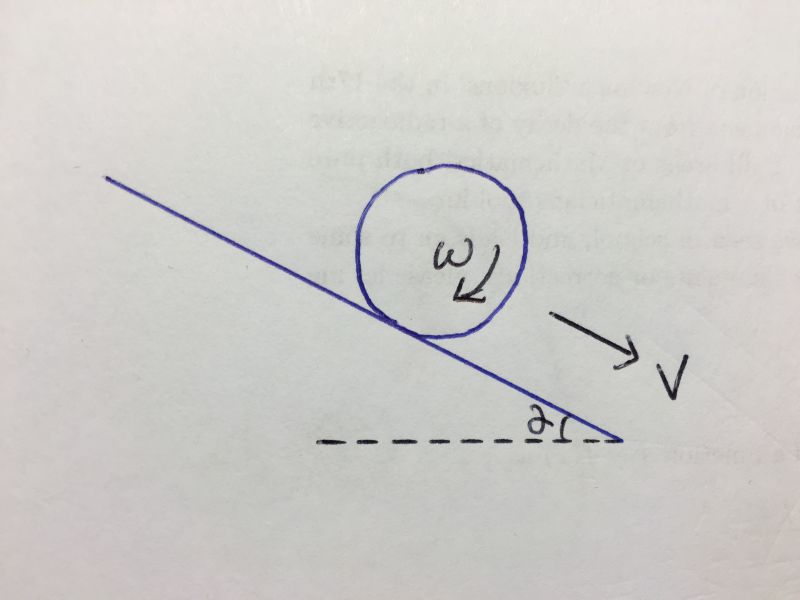
\includegraphics[scale=0.20]{Rel14})\\

In terms of forces and torques:
\begin{equation*}
\begin{aligned}
M\dot{v}&=Mg\sin\alpha-F\\
I\dot{\omega}&=aF
\end{aligned}
\end{equation*}
While rolling, $\dot{v}-a\dot{\omega}=0$. Thus
\begin{equation*}
\begin{aligned}
M\dot{v}=Mg\sin\alpha-\frac{I}{a^2}\dot{v}
\end{aligned}
\end{equation*}
leading to the same result. Here $F$ is a \emph{static} frictional force. It does no work (so energy is conserved) because $v_{slip}=0$.

\begin{eg}(snooker ball)\\
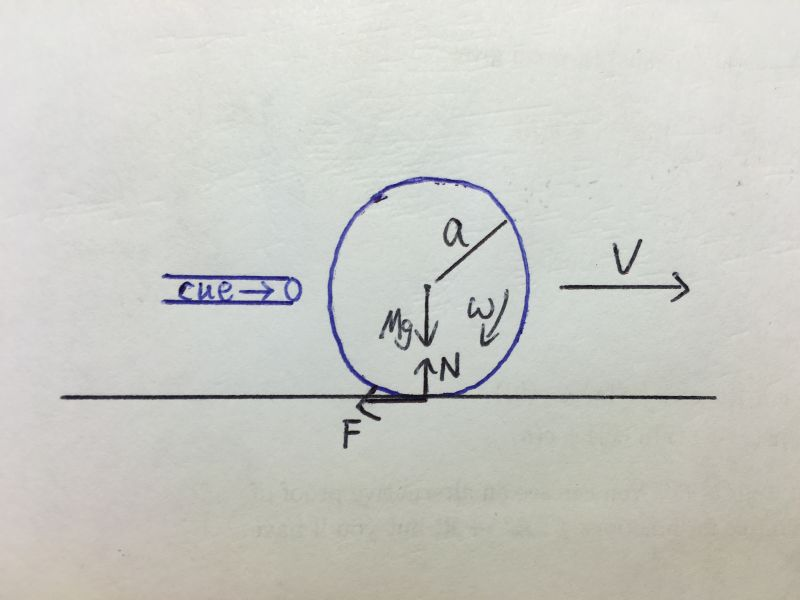
\includegraphics[scale=0.20]{Rel16}\\
Struck centrally so as to initiate translation but no rotation. Sliding occurs initially.\\
Constant frictional force
\begin{equation*}
\begin{aligned}
F=\mu_k Mg
\end{aligned}
\end{equation*}
applies while $v-a\omega >0$. ($\mu_k$: coefficient of kinetic friction)\\
Moment of inertia is
\begin{equation*}
\begin{aligned}
I=\frac{2}{5}Ma^2
\end{aligned}
\end{equation*}
about centre of mass.\\
Equations of motion:
\begin{equation*}
\begin{aligned}
&M\dot{v}=-F\\
&I\dot{\omega}=aF
\end{aligned}
\end{equation*}
Initially $v=v_0$ and $\omega =0$.\\
Solution:
\begin{equation*}
\begin{aligned}
&v=v_0-\mu_k gt\\
&\omega=\frac{5}{2}\frac{\mu_k g}{a}t
\end{aligned}
\end{equation*}
Slipping velocity
\begin{equation*}
\begin{aligned}
v_{slip} &= v-a\omega\\
&= v_0 - \frac{7}{2}\mu_k gt\\
&= v_0 \left(1-\frac{t}{t_{roll}}\right)
\end{aligned}
\end{equation*}
where
\begin{equation*}
\begin{aligned}
t_{roll} = \frac{2}{7}\frac{v_0}{\mu_k g}.
\end{aligned}
\end{equation*}
The solution applies until $t=t_{roll}$, at which time rolling begins and friction ceases.\\
At this point,
\begin{equation*}
\begin{aligned}
v=a\omega = \frac{5}{7}v_0
\end{aligned}
\end{equation*}
The kinetic energy is
\begin{equation*}
\begin{aligned}
\frac{1}{2}Mv^2 + \frac{1}{2}I\omega^2 &= \frac{1}{2}\left(1+\frac{2}{5}\right)Mv^2\\
&=\frac{5}{14}Mv_0^2 < \frac{1}{2}Mv_0^2
\end{aligned}
\end{equation*}
So energy has been lost to friction.
\end{eg}

\newpage
\section{Special relativity}
When particles move extremely fast, Newtonian Dynamics becomes inaccurate and is replaced by Einstein's Special Theory of Relativity (1905).\\
Its effects are noticeable only when particles approach the speed of light,
\begin{equation*}
\begin{aligned}
c=299792458 ms^{-1} \approx 3\times 10^8 ms^{-1}
\end{aligned}
\end{equation*}
The Special Theory of Relativity rests on two postulates:\\
$\bullet$ Postulate 1: The laws of physics are the same in all inertial frames (the principle of relativity, as considered by Galileo).\\
$\bullet$ Postulate 2: The speed of light in vacuum is the same in all inertial frames.\\
The second postulate is not compatible with Galilean relativity and requires a complete revision of our ideas about space and time.\\

Consider two inertial frames, $S$ and $S'$, related by the Galilean transformation
\begin{equation*}
\begin{aligned}
x'&=x-vt\\
y'&=y\\
z'&=z\\
t'&=t
\end{aligned}
\end{equation*}
In $S$, a light ray (or photon) travels in the $x$ direction with speed $c$. Its trajectory is
\begin{equation*}
\begin{aligned}
\frac{x}{t}=c.
\end{aligned}
\end{equation*}
The Galilean transformation gives
\begin{equation*}
\begin{aligned}
\frac{x'}{t'}=\frac{x-vt}{t}=c-v
\end{aligned}
\end{equation*}
So the speed of light in $S'$ would be $c-v$. How can this common sense result be wrong?

\subsection{The Lorentz transformation}
\subsubsection{The Lorentz transformation}
Consider again inertial frames $S$ and $S'$ in standard configuration. Assume that the origins coincide at $t=t'=0$.\\
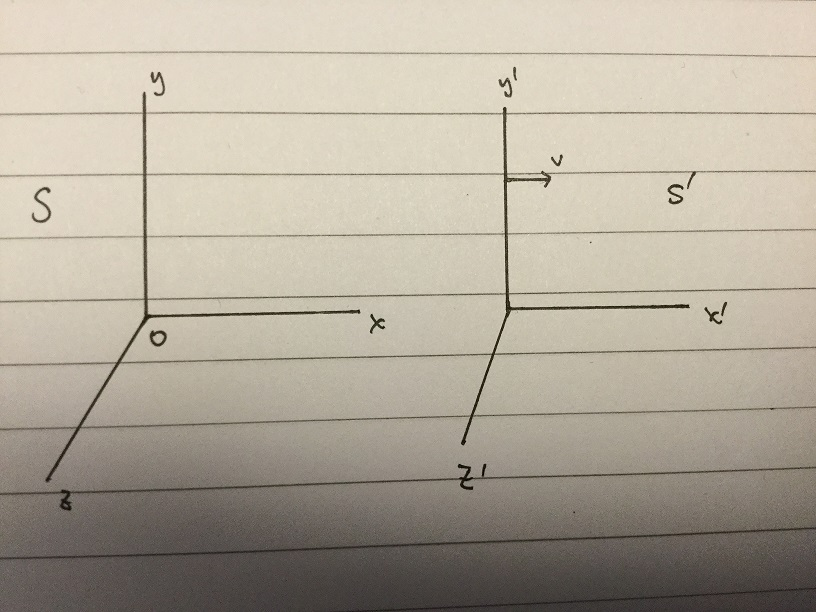
\includegraphics[scale=0.25]{Rel17}\\
For now, neglect $y$ and $z$, and consider the relationship between $\left(z,t\right)$ and $\left(x',t'\right)$.\\
The most general form is
\begin{equation*}
\begin{aligned}
x'=f\left(x,t\right)\\
t'=g\left(x,t\right)
\end{aligned}
\end{equation*}
for some functions $f$ and $g$.\
In any inertial frame, a free particle moves with constant velocity. Straight lines in $\left(x,t\right)$ must map into straight lines in $\left(x',t'\right)$. Therefore the relationship must be linear.\\
Given that the origins of $S$ and $S'$ coincide (at $t=t'=0$) and $S'$ moves with velocity $v$ relative to $S$, the line $x=vt$ must map into $x'=0$.\\
Therefore
\begin{equation}\label{eq:1}
\begin{aligned}
x'=\gamma \left(x-vt\right)
\end{aligned}
\end{equation}
for some factor $\gamma$ that may depend on $|v|$.
Now reverse the roles of the two frames.\\
From the perspective of $S'$, $S$ moves with velocity $-v$. A similar argument leads to
\begin{equation}\label{eq:2}
\begin{aligned}
x=\gamma\left(x'+vt\right)
\end{aligned}
\end{equation}
with the same $\gamma$ since it only depends on $|v|$.\\
Now consider a light ray (or photon) passing through the origin $x=x'=0$ at $t=t'=0$. Its trajectory in $S$ is
\begin{equation*}
\begin{aligned}
x=ct
\end{aligned}
\end{equation*}
We demand that its trajectory in $S'$ be
\begin{equation*}
\begin{aligned}
x'=ct'
\end{aligned}
\end{equation*}
so that the speed of light is the same in each frame.\\
Substituting these equations into (\ref{eq:1}) and (\ref{eq:2}), we have
\begin{equation*}
\begin{aligned}
ct' = \gamma \left(c-v\right)t
\end{aligned}
\end{equation*}
and
\begin{equation*}
\begin{aligned}
ct = \gamma \left(c+v\right) t'
\end{aligned}
\end{equation*}
So
\begin{equation*}
\begin{aligned}
&c^2 = \gamma^2 \left(c^2-v^2\right)\\
\implies &\gamma = \frac{1}{\sqrt{1-\frac{v^2}{c^2}}}
\end{aligned}
\end{equation*}
This is the \emph{Lorentz factor} $\gamma\left(v\right)$.

Note that:
$\bullet$ $\gamma \geq 1$ is an increasing function of $|v|$;\\
$\bullet$ when $|v| \ll c$, $\gamma \approx 1$ and we recover the Galilean transformation;\\
$\bullet$ when $|v| \to c$, $r\to\infty$;\\
$\bullet$ when $|v| > c$, $\gamma$ is imaginary, which is impossible.\\
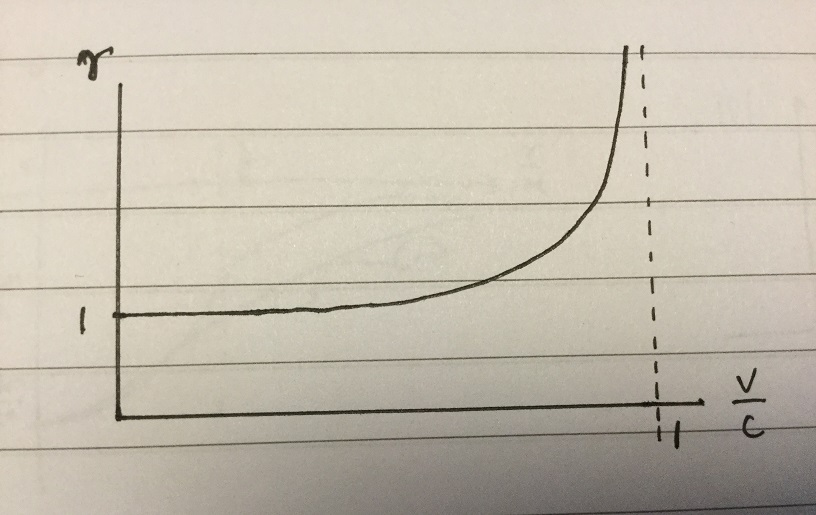
\includegraphics[scale=0.20]{Rel18}\\
($\gamma = 2$ when $\frac{v}{c} \approx 0.866$,\\
$\gamma = 5$ when $\frac{v}{c} \approx 0.980$,\\
$\gamma = 10$ when $\frac{v}{c} \approx 0.995$,\\
$\gamma = 20$ when $\frac{v}{c} \approx 0.999$.)\\
Eliminate $x'$ between (\ref{eq:1}) and (\ref{eq:2}):
\begin{equation*}
\begin{aligned}
x&=\gamma \left(\gamma \left(x-vt\right)+vt'\right)\\
\implies t'&=\gamma t-\left(1-\frac{1}{\gamma^2}\right) \frac{\gamma x}{v}\\
&= \gamma t - \frac{\gamma v}{c^2}x
\end{aligned}
\end{equation*}
The equations
\begin{equation*}
\begin{aligned}
x'=\gamma\left(x-vt\right), t'=\gamma\left(t-\frac{v}{c^2}x\right)
\end{aligned}
\end{equation*}
represent the \emph{Lorentz transformation} in standard configuration (in one spatial dimension). In the limit $\frac{v}{c}\to 0$ ($\gamma \to 1$), they reduce to the Galilean transformation.\\
We can invert this linear mapping to find (after some algebra)
\begin{equation*}
\begin{aligned}
x=\gamma\left(x'+vt'\right), t=\gamma\left(t'+\frac{v}{c^2}x'\right)
\end{aligned}
\end{equation*}
i.e. the same but with $v\to -v$.\\
Directions perpendicular to the relative motion of the frames are unaffected:
\begin{equation*}
\begin{aligned}
y'=y, z'=z
\end{aligned}
\end{equation*}

\subsubsection{Checking the speed of light}
For a light ray travelling in the $x$ direction in $S$:\\
In $S$:
\begin{equation*}
\begin{aligned}
x=ct, y=0, z=0
\end{aligned}
\end{equation*}
In $S'$:
\begin{equation*}
\begin{aligned}
\frac{x'}{t'}=\frac{\gamma\left(x-vt\right)}{\gamma\left(t-\frac{v}{c^2}x\right)} - \frac{\left(c-v\right)t}{\left(1-\frac{v}{c}\right)t} = c
\end{aligned}
\end{equation*}
and $y'=0$, $z'=0$ as required.\\

For a light ray travelling in the $y$ direction in $S$:\\
In $S$:
\begin{equation*}
\begin{aligned}
x=0,y=ct,z=0
\end{aligned}
\end{equation*}
In $S'$:
\begin{equation*}
\begin{aligned}
&\frac{x'}{t'}=\frac{\gamma\left(x-vt\right)}{\gamma\left(t-\frac{v}{c^2}x\right)} = -v\\
&\frac{y'}{t'}=\frac{y}{\gamma\left(t-\frac{v}{c^2}x\right)}=\frac{c}{\gamma}\\
&z'=0\\
\implies &\frac{\sqrt{x'^2 + y'^2}}{t} = \sqrt{v^2 + \frac{c^2}{\gamma^2}}=c
\end{aligned}
\end{equation*}
as required.\\

More generally, the Lorentz transformation implies
\begin{equation*}
\begin{aligned}
c^2 t'^2 - r'^2 &= c^2 t'^2 - x'^2 - y'^2 - z'^2\\
&= c^2 \gamma^2\left(t-\frac{v}{c^2}x\right)^2 - \gamma^2\left(x-vt\right)^2 - y^2 - z^2\\
&=\gamma^2 \left(1-\frac{v^2}{c^2}\right)\left(c^2 t^2 - x^2\right) - y^2 - z^2\\
&=c^2 t^2 - x^2 - y^2 - z^2\\
&=c^2 t^2 - r^2
\end{aligned}
\end{equation*}
So, if $\frac{r}{t}=c$, then $\frac{r'}{t'}=c$ as well.

\subsubsection{Space-time diagrams}
When considering one spatial dimension ($x$) and time($t$) in an inertial frame $S$, we plot $x$ on the horizontal axis and $ct$ on the vertical axis.\\
(diagram to be inserted -- rel19)\\
The union of space and time in special relativity is called \emph{Minkowski spacetime}.\\
Each point $p$ represents an \emph{event}, labelled by coordinates $\left(ct,x\right)$.\\
A particle traces out a \emph{world line} in spacetime, which is straight if the particle moves uniformly.\\
Light rays moving in the $x$ direction have world lines inclined at $45^\circ$.\\
We will see later that particles cannot travel with speed $v>c$.\\
(diagram to be inserted -- rel20)\\
We can also draw the axes of $S'$, moving with velocity $v$ in the $x$ direction relative to $S$.\\
The $t'$ axis corresponds to $x'=0$, i.e.
\begin{equation*}
\begin{aligned}
x=\frac{v}{c}ct
\end{aligned}
\end{equation*}
The $x'$ axis corresponds to $t'=0$, i.e.
\begin{equation*}
\begin{aligned}
ct = \frac{v}{c}x
\end{aligned}
\end{equation*}
(these are simply obtained by the previous Lorentz transformation equations)\\
(diagram to be inserted -- rel 21)\\
The axes are symmetric about the diagonal. This reflects the fact that the speed of light in $S'$ is also $c$.

\subsection{Relativity physics}
\subsubsection{Simultaneity}
Two events $P_1$ and $P_2$ are \emph{simultaneous} in the frame $S$ if $t_1 = t_2$.\\
(diagram to be inserted -- rel22)\\
However, events that are simultaneously in $S'$ have equal values of $t'$, and so they lie in lines
\begin{equation*}
\begin{aligned}
ct-\frac{v}{c}x=\text{   constant}
\end{aligned}
\end{equation*}
(diagram to be inserted -- rel23)\\
Therefore \emph{simultaneity is relative}.

\subsubsection{Causality}
Although differently moving observers may disagree on the temporal ordering of events, the consistent ordering of cause and effect can be ensured.\\
Lines of simultaneity cannot be inclined at more than $45^\circ$, because Lorentz boosts are possible only for $|v|<c$.\\
(diagram to be inserted -- rel24)\\
The lines at $45^\circ$ emerging from $P$ from the \emph{past light cone} and \emph{future light cone} of $P$.\\
All observers agree that $Q$ occurs after $P$. Different observers may disagree on the temporal ordering of $P$ and $R$.\\
If nothing can travel faster than light, than $P$ and $R$ cannot influence each other.\\
$P$ can only influence events within its future light cone, and $P$ can only be influenced by events within its past light cones.

\subsubsection{Time dilation}
A clock that is stationary in $S'$ ticks at constant intervals $\triangle t'$.\\
What is the interval between ticks in $S$?\\
The inverse Lorentz transformation gives
\begin{equation*}
\begin{aligned}
t = \gamma\left(t'+\frac{v}{c^2}x'\right)
\end{aligned}
\end{equation*}
Since $x'$ is constant for the clock, we have
\begin{equation*}
\begin{aligned}
\triangle t = \gamma \triangle t' > \triangle t'
\end{aligned}
\end{equation*}
Therefore \emph{moving clocks run slowly}.

\begin{defi} (Proper time)\\
\emph{Proper time} is the time measured in an object's rest frame.
\end{defi}

\subsubsection{The twin paradox}
Consider two twins: Luke and Leia. Luke stays at home while Leia travels at constant speed $v$ to a distant planet $P$, then turns around and returns at the same speed.\\
(diagram to be inserted -- rel25)\\
Leia's arrival(A) at $P$ has
\begin{equation*}
\begin{aligned}
\left(ct,x\right) = \left(cT,vT\right).
\end{aligned}
\end{equation*}
The time experienced by Leia on her outward journey is
\begin{equation*}
\begin{aligned}
T' = \gamma \left(T-\frac{v}{c^2}vT\right) = \frac{T}{\gamma}
\end{aligned}
\end{equation*}
By Leia's return (R), Luke has aged by $2T$, but Leia has aged by $\frac{2T}{\gamma}<2T$ so she is younger than Luke because of time dilation.\\
Paradox: from Leia's perspective, Luke travelled away from her at speed $v$ and then returned, so he should be younger than her!\\
Why is the problem not symmetric?\\
(diagram to be inserted -- rel26)\\
In the frame of reference of Leia's outward journey, her arrival $A$ is simultaneous with Luke's event $X$, which has $x=0$ and $t'=T'=\frac{T}{\gamma}$. So
\begin{equation*}
\begin{aligned}
t' = \gamma\left(t-\frac{v}{c^2}x\right) \implies t=\frac{T'}{\gamma}=\frac{T}{\gamma^2}
\end{aligned}
\end{equation*}
This is how much Luke has aged from Leia's perspective when she arrives at $P$.\\
At this stage the problem is symmetric: each thinks the other has aged less by a factor of $\frac{1}{\gamma}$.\\
Things change when Leia turns around and changes frame of reference. Suppose Leia meets a friend Han who is just leaving $P$ at speed $v$.\\
(diagram to be inserted -- rel27)\\
On his journey, Han thinks that Luke ages by $\frac{T}{\gamma^2}$. But in his frame of reference, his departure is simultaneous with Luke's event $Z$.\\
The asymmetry between Luke and Leia occurs when Leia turns around.\\
At this point she sees Luke age rapidly from $X$ to $Z$.

\subsubsection{Length contraction}
Suppose we have a rod of length $L'$ stationary in frame $S'$. What is its length in frame $S$?\\
In $S'$:\\
(diagram to be inserted -- rel28)\\
The length of the rod is the distance between the two ends at the same time!\\
In frame $S$:\\
(diagram to be inserted -- rel29)\\
The lines $x'=0$ and $x'=L'$ map into (using the Lorentz transformation $x'=\gamma\left(x-vt\right)$):
\begin{equation*}
\begin{aligned}
x=vt, x=vt+\frac{L'}{\gamma}
\end{aligned}
\end{equation*}
So the length in $S$ is
\begin{equation*}
\begin{aligned}
L=\frac{L'}{\gamma} < L'
\end{aligned}
\end{equation*}
Therefore \emph{moving objects are contracted in the direction of motion}.

\begin{defi} (Proper length)\\
The \emph{proper length} is the length measured in an object's rest frame.
\end{defi}

Does a train of length $2L$ fit alongside a platform of length $L$ if it travels through the station at a speed $v$ such that $\gamma=2$?\\
For the system of observers on the platform, the train contracts to a length $\frac{2L}{\gamma} = L$. So it fits!\\
But for the system of observers on the train, the platform contracts to a length $\frac{L}{\gamma} = \frac{L}{2}$, which is much too short!\\
(diagram to be inserted -- rel30)\\
No paradox here -- lengths are different because simultaneity is relative.

\subsubsection{Composition of velocities}
A particle moves with constant velocity $u'$ in frame $S'$, which moves with velocity $v$ relative to $S$.\\
What is its velocity $u$ in $S$?\\
The world line of the particle in $S'$ is
\begin{equation*}
\begin{aligned}
x' = u't'
\end{aligned}
\end{equation*}
In $S$,
\begin{equation*}
\begin{aligned}
u=\frac{x}{t}&=\frac{\gamma\left(x'+vt'\right)}{\gamma\left(t'+\frac{v}{c^2}x'\right)}\\
&=\frac{u't'+vt'}{t'+\frac{v}{c^2}u't'}\\
&=\frac{u'+v}{1+\frac{u'v}{c^2}}
\end{aligned}
\end{equation*}
This is the formula for the relativistic composition of parallel velocities.\\
The inverse transformation is found by swapping $u$ and $u'$ and changing the sign of $v$.\\
Note that:\\
$\bullet$ When $u'v \ll c^2$, it reduces to the standard Galilean addition of velocities.\\
$\bullet$ For given $v$ ($|v|<c$ always) $u$ is a monotonically increasing function of $u'$.\\
$\bullet$ When $u'=\pm c$, $u=u'$ for any $v$.\\
$\bullet$ Therefore, when $|u'|<c$, $|u|<c$ also.\\
(You cannot reach or exceed light speed by any combination of boosts.)\\
(diagram to be inserted -- rel31)

\subsection{Geometry of spacetime}
\subsubsection{The invariant interval}
Consider events $P$ and $Q$ with coordinates $\left(ct_1,x_1\right)$ and $\left(ct_2,x_2\right)$ separated by
\begin{equation*}
\begin{aligned}
\triangle t = t_2 - t_1, \triangle x = x_2 - x_1
\end{aligned}
\end{equation*}
The \emph{invariant interval} between $P$ and $Q$ is defined as
\begin{equation*}
\begin{aligned}
\triangle s^2 = c^2 \triangle t^2 - \triangle x^2
\end{aligned}
\end{equation*}
All inertial observers agree on the value of $\triangle s^2$:
\begin{equation*}
\begin{aligned}
c^2 \triangle t'^2 -\triangle x'^2 &= c^2 \gamma^2 \left(\triangle t-\frac{v}{c^2}\triangle x\right)^2 - \gamma^2 \left(\triangle x-v\triangle t\right)^2\\
&= \gamma^2 \left(1-\frac{v^2}{c^2}\right)\left(c^2\triangle t^2 - \triangle x^2\right)\\
&= c^2 \triangle t^2 - \triangle x^2
\end{aligned}
\end{equation*}
In three spatial dimensions, the invariant interval is
\begin{equation*}
\begin{aligned}
\triangle s^2 = c^2 \triangle t^2 - \triangle x^2 - \triangle y^2 - \triangle z^2
\end{aligned}
\end{equation*}
For two infinitesimally separated events, we have the \emph{line elements}
\begin{equation*}
\begin{aligned}
ds^2 = c^2dt^2 - dx^2 - dy^2 - dz^2
\end{aligned}
\end{equation*}
Spacetime is topologically equivalent to $\R^4$. When endowed with the distant measure $\triangle s^2$ (which is not positive definite), it is called the \emph{Minkowski spacetime}.\\
We say it has dimension $d=1+3$.\\
Events with $\triangle s^2 > 0$ are \emph{timelike separated}.\\
(There is a frame in which they occur at the same position).\\
(diagram to be inserted -- rel32)\\
Events with $\triangle s^2 < 0$ are \emph{spacelike separated}.\\
(There is a frame in which they occur at the same time).\\
(diagram to be inserted -- rel33)\\
Event with $\triangle s^2=0$ are \emph{lightlike separated} (or \emph{null separated}). (They could be connected by a light ray).\\
(diagram to be inserted -- rel34)\\
(Note that $\triangle s^2 = 0$ does not imply that $P$ and $Q$ are the same event.)

\subsubsection{The Lorentz group}
The coordinates of an event $P$ in frame $S$ can be written as a \emph{4-vector} (4-component vector) $X$.
\begin{equation*}
\begin{aligned}
X^\mu = \left(
\begin{array}{ll}
ct\\
x\\
y\\
z
\end{array}
\right), \mu = 0,1,2,3
\end{aligned}
\end{equation*}
The invariant interval between the origin and $P$ can be written as an inner product
\begin{equation*}
\begin{aligned}
X\cdot X = X^T \eta X = X^\mu \eta_{\mu\mu} X^\mu
\end{aligned}
\end{equation*}
(summation convention) where
\begin{equation*}
\begin{aligned}
\eta = \left(
\begin{matrix}
1&0&0&0\\
0&-1&0&0\\
0&0&-1&0\\
0&0&0&-1
\end{matrix}
\right)
\end{aligned}
\end{equation*}
is the \emph{Minkowski metric}.\\
We see that
\begin{equation*}
\begin{aligned}
X\cdot X = c^2 t^2 - x^2 - y^2 - z^2
\end{aligned}
\end{equation*}
as required.\\

4-vectors with $X\cdot X > 0$ are called timelike;\\
4-vectors with $X\cdot X < 0$ are called spacelike;\\
4-vectors with $X\cdot X = 0$ are called lightlike.\\

A Lorentz transformation is a linear transformation of the coordinates from one frame $\left(S\right)$ to another $\left(S'\right)$, represented by a $4\times 4$ matrix:
\begin{equation*}
\begin{aligned}
X' = \Lambda X
\end{aligned}
\end{equation*}
Lorentz transformations can be defined as those that leave the inner product invariant:
\begin{equation*}
\begin{aligned}
X' \cdot X' = X \cdot X
\end{aligned}
\end{equation*}
for all $X$, which implies the matrix equation
\begin{equation*}
\begin{aligned}
\Lambda^T \eta \Lambda = \eta
\end{aligned}
\end{equation*}
Two classes of solution of this equation are:\\
1)
\begin{equation*}
\begin{aligned}
\Lambda = \left(
\begin{matrix}
1&0&0&0\\
0& & &\\
0& &R&\\
0& & &
\end{matrix}
\right)
\end{aligned}
\end{equation*}

With $R$ a $3\times 3$ matrix satisfying
\begin{equation*}
\begin{aligned}
R^T R = I
\end{aligned}
\end{equation*}
These are spatial rotations (improper, since they include reflections).\\
2)
\begin{equation*}
\begin{aligned}
\Lambda = \left(
\begin{matrix}
\gamma & -\gamma\beta & 0&0\\
-\gamma\beta & \gamma & 0&0\\
0&0&1&0\\
0&0&0&1
\end{matrix}
\right)
\end{aligned}
\end{equation*}
where we define
\begin{equation*}
\begin{aligned}
\beta = \frac{v}{c}, \gamma = \frac{1}{\sqrt{1-\beta^2}}
\end{aligned}
\end{equation*}
These are Lorentz boosts in the $x$ direction.\\

The set of all matrices satisfying
\begin{equation*}
\begin{aligned}
\Lambda^T \eta \Lambda = \eta
\end{aligned}
\end{equation*}
form the \emph{Lorentz group} $O\left(1,3\right)$. It is generated by rotations and boosts, and includes spatial reflections and time reversals.\\
The subgroup with $\det \Lambda = +1$ is the \emph{proper Lorentz group} $SO\left(1,3\right)$;\\
The subgroup that preserves spatial orientation and the direction of time is the \emph{restricted Lorentz group} $SO^+ \left(1,3\right)$.

\subsubsection{Rapidity}
Focus on the upper $2\times 2$ matrix of Lorentz boosts in the $x$ direction.\\
Write
\begin{equation*}
\begin{aligned}
\Lambda\left[\beta\right] = \left(
\begin{matrix}
\gamma & -\gamma\beta\\
-\gamma\beta & \gamma
\end{matrix}\right)
\end{aligned}
\end{equation*}
with
\begin{equation*}
\begin{aligned}
\gamma = \frac{1}{\sqrt{1-\beta^2}}
\end{aligned}
\end{equation*}
Combining two boosts in the $x$ direction, we have
\begin{equation*}
\begin{aligned}
\Lambda\left[\beta_1\right] \Lambda \left[\beta_2\right]& = 
\left(\begin{matrix}
\gamma_1 & -\gamma_1 \beta_1\\
-\gamma_1 \beta_1 & \gamma_1
\end{matrix}\right)
\left(\begin{matrix}
\gamma_2 & -\gamma_2 \beta_2\\
-\gamma_2 \beta_2 & \gamma_2
\end{matrix}\right)\\
&=\Lambda\left[\frac{\beta_1 + \beta_2}{1+\beta_1 \beta_2}\right]
\end{aligned}
\end{equation*}
after \emph{some} messy algebra. This is just the velocity composition formula in dimensionless form.\\
Recall that, for spatial rotations,
\begin{equation*}
\begin{aligned}
R\left(\theta\right) = \left(\begin{matrix}
\cos\theta & \sin\theta\\
-\sin\theta & \cos\theta
\end{matrix}\right)
\end{aligned}
\end{equation*}
and
\begin{equation*}
\begin{aligned}
R\left(\theta_1\right) R\left(\theta_2\right) = R\left(\theta_1 + \theta_2\right)
\end{aligned}
\end{equation*}
For Lorentz boosts, define the \emph{rapidity} $\phi$ such that
\begin{equation*}
\begin{aligned}
\beta = \tanh\phi, \gamma = \cosh \phi, \gamma\beta = \sinh \phi
\end{aligned}
\end{equation*}
Then
\begin{equation*}
\begin{aligned}
\Lambda\left[\beta\right] = \left(\begin{matrix}
\cosh\phi & \sinh\phi\\
-\sinh\phi & \cosh\phi
\end{matrix}\right)=\Lambda\left(\phi\right)
\end{aligned}
\end{equation*}
and the rapidities add like rotation angles:
\begin{equation*}
\begin{aligned}
\Lambda\left(\phi_1\right) \Lambda \left(\phi_2\right) = \Lambda \left(\phi_1+\phi_2\right)
\end{aligned}
\end{equation*}
This shows the close relationship between rotations and boosts. A boost is a hyperbolic notation in spacetime.

\subsection{Relativistic kinematics}
A particle moves along a trajectory $\mathbf{x}\left(t\right)$ in $S$. Its velocity is
\begin{equation*}
\begin{aligned}
\mathbf{u}\left(t\right) = \frac{d\mathbf{x}}{dt}
\end{aligned}
\end{equation*}
However, there is a better way to describe its trajectory.\\
\subsubsection{Proper time}
First consider a particle at rest in an inertial frame $S'$ with $\mathbf{x}' = \mathbf{0}$. The invariant interval between points on its world line is
\begin{equation*}
\begin{aligned}
\triangle s^2 = c^2 \triangle t'^2
\end{aligned}
\end{equation*}
Define \emph{proper time} $\tau$ such that
\begin{equation*}
\begin{aligned}
\triangle \tau = \frac{\triangle s}{c}
\end{aligned}
\end{equation*}
This is the time experienced by the particle. But the equation
\begin{equation*}
\begin{aligned}
\triangle \tau = \frac{\triangle s}{c}
\end{aligned}
\end{equation*}
holds in all fames, because $\triangle s$ is Lorentz-invariant (and real for particles that travel slower than light).\\
The world line of a particle can be parameterised using the proper time $\tau$: $\mathbf{x}\left(\tau\right)$ and $t\left(\tau\right)$:\\
(diagram to be inserted -- rel35)\\
Infinitesimal changes are related by
\begin{equation*}
\begin{aligned}
d\tau &= \frac{ds}{c}\\
&=\frac{\sqrt{c^2dt^2 - |d\mathbf{x}|^2}}{c}\\
&=\sqrt{1-\frac{|\mathbf{u}|^2}{c^2}} dt
\end{aligned}
\end{equation*}
Thus
\begin{equation*}
\begin{aligned}
\frac{dt}{d\tau} = \gamma_u
\end{aligned}
\end{equation*}
with
\begin{equation*}
\begin{aligned}
\gamma_u = \frac{1}{\sqrt{1-\frac{|\mathbf{u}|}{c^2}}}
\end{aligned}
\end{equation*}
The total time experienced by the particle along a segment of its world line is
\begin{equation*}
\begin{aligned}
T=\int d\tau = \int \frac{dt}{\gamma_u}
\end{aligned}
\end{equation*}

\subsubsection{4-velocity}
The \emph{position 4-vector} of a particle is
\begin{equation*}
\begin{aligned}
X\left(\tau\right) = \left(\begin{matrix}
ct\left(\tau\right)\\
\mathbf{x}\left(\tau\right)
\end{matrix}\right)
\end{aligned}
\end{equation*}
Its \emph{4-velocity is defined as}
\begin{equation*}
\begin{aligned}
U = \frac{dX}{d\tau} &= \left(\begin{matrix}
c\frac{dt}{d\tau}\\\\
\frac{d\mathbf{x}}{d\tau}
\end{matrix}\right)\\
&= \frac{dt}{d\tau} \left(\begin{matrix}
c\\
\mathbf{u}
\end{matrix}\right)\\
&=\gamma_u\left(\begin{matrix}
c\\
\mathbf{u}
\end{matrix}\right)
\end{aligned}
\end{equation*}
where 
\begin{equation*}
\begin{aligned}
\mathbf{u} = \frac{d\mathbf{x}}{dt}
\end{aligned}
\end{equation*}

Another common notation is
\begin{equation*}
\begin{aligned}
X=\left(ct,\mathbf{x}\right), U=\gamma_u\left(c,\mathbf{u}\right)
\end{aligned}
\end{equation*}

If frame $S$ and $S'$ are related by
\begin{equation*}
\begin{aligned}
X' = \Lambda X
\end{aligned}
\end{equation*}
then the 4-velocity also transforms as
\begin{equation*}
\begin{aligned}
U' = \Lambda U
\end{aligned}
\end{equation*}

Any 4-component vector that transforms in this way under a Lorentz transformation is called a 4-vector. $U$ is a 4-vector because $X$ is a 4-vector and $\tau$ is Lorentz-invariant. Note that $\frac{dX}{dt}$ is \emph{not} a 4-vector.\\

The inner product
\begin{equation*}
\begin{aligned}
U \cdot U = U' \cdot U'
\end{aligned}
\end{equation*}
is a Lorentz invariant, which is the same in all inertial frames.\\
In the rest frame of the particle,
\begin{equation*}
\begin{aligned}
U= \left(\begin{matrix}
c\\
\mathbf{0}
\end{matrix}\right) \implies U\cdot U = c^2
\end{aligned}
\end{equation*}
In any other frame,
\begin{equation*}
\begin{aligned}
U&=\gamma_u \left(\begin{matrix}
c\\
\mathbf{u}
\end{matrix}\right)\\
\implies U\cdot U &= \gamma_u^2 \left(c^2-u^2\right)\\
&= c^2
\end{aligned}
\end{equation*}
again as expected.

\subsubsection{Transformation of velocities revisited}
We've seen that velocities cannot simply be added in relativity. However, the 4-velocity does transform linearly according to the Lorentz transformation
\begin{equation*}
\begin{aligned}
U' = \Lambda U
\end{aligned}
\end{equation*}
In frame $S$, consider a particle moving at speed $u$ at angle $\theta$ to the $x$ axis in the $xy$ plane.\\
(diagram rel-36)\\
Its 4-velocity is
\begin{equation*}
\begin{aligned}
U=\left(\begin{matrix}
\gamma_u c\\
\gamma_u u\cos \theta\\
\gamma_u u\sin \theta\\
0
\end{matrix}\right)
\end{aligned}
\end{equation*}
with
\begin{equation*}
\begin{aligned}
\gamma_u = \frac{1}{\sqrt{1-\frac{u^2}{c^2}}}.
\end{aligned}
\end{equation*}
With frames $S$ and $S'$ in standard configuration,
\begin{equation*}
\begin{aligned}
\left(\begin{matrix}
\gamma_{u'} c\\
\gamma_{u'}u'\cos\theta'\\
\gamma_{u'}u'\sin\theta'\\
0
\end{matrix}\right)
=
\left(\begin{matrix}
\gamma_v & -\gamma_v \frac{v}{c} & 0 & 0\\
-\gamma_v\frac{v}{c} & \gamma_v & 0 & 0\\
0&0&1&0\\
0&0&0&1
\end{matrix}\right)
\left(\begin{matrix}
\gamma_u c\\
\gamma_u u\cos\theta\\
\gamma_u u\sin\theta\\
0
\end{matrix}\right)
\end{aligned}
\end{equation*}
(diagram rel-37)\\
The ration of the second and first lines $\left(x c\right)$ gives
\begin{equation*}
\begin{aligned}
u'\cos\theta' = \frac{u\cos\theta - v}{1-\frac{uv}{c^2}\cos\theta}
\end{aligned}
\end{equation*}
just like the composition of parallel velocities.\\
The ratio of the thirs and second lines is
\begin{equation*}
\begin{aligned}
\tan \theta' = \frac{u\sin \theta}{\gamma_v \left(u\cos\theta - v\right)}
\end{aligned}
\end{equation*}
which describes \emph{aberration}: a change in the apparent direction of motion of a particle due to the motion of the observer.\\
Aberration of starlight ($u=c$) due to the Earth's orbital motion causes small annual changes in the apparent positions of stars.

\subsubsection{4-momentum}
The \emph{4-momentum} of a particle of mass $m$ is
\begin{equation*}
\begin{aligned}
P=mU=m\gamma_u \left(
\begin{array}{ll}
c\\
\mathbf{u}
\end{array}\right)
\end{aligned}
\end{equation*}
with
\begin{equation*}
\begin{aligned}
\gamma_u = \frac{1}{\sqrt{1-\frac{|\mathbf{u}|^2}{c^2}}}
\end{aligned}
\end{equation*}
The 4-momentum of a system of particles is the sum of the 4-momentum of the particles, and is conserved in the absence of external forces.\\
The spatial components of $P$ are the \emph{relativistic 3-momentum}
\begin{equation*}
\begin{aligned}
\mathbf{p} = m\gamma_u\mathbf{u}
\end{aligned}
\end{equation*}
which differs from the Newtonian expression by a factor of $\gamma_u$.\\
Note that $|\mathbf{p}| \to \infty$ as $|\mathbf{u}| \to c$.\\
What is the interpretation of the time-component $p^\circ$? Expand for $|\mathbf{u}| \ll c$:
\begin{equation*}
\begin{aligned}
p^\circ = m\gamma_u c &= \frac{mc}{\sqrt{1-\frac{|\mathbf{u|^2}}{c^2}}}\\
&=\frac{1}{c}\left(mc^2+\frac{1}{2}m|\mathbf{u}|^2+...\right)
\end{aligned}
\end{equation*}
Since $p^\circ$ is conserved, this strongly suggests that we should interpret $P$ as
\begin{equation*}
\begin{aligned}
P = \left(
\begin{array}{ll}
\frac{E}{c}\\
\mathbf{p}
\end{array}\right)
\end{aligned}
\end{equation*}
where $E$ is the \emph{relativistic energy}.\\
Then
\begin{equation*}
\begin{aligned}
E&=m\gamma_u c^2\\
&=mc^2 + \frac{1}{2}m|\mathbf{u}|^2 + ...
\end{aligned}
\end{equation*}
for $|\mathbf{u}| \ll c$.\\
Note that $E\to \infty$ as $|\mathbf{u}| \to c$.\\
For a stationary particle,
\begin{equation*}
\begin{aligned}
E=mc^2
\end{aligned}
\end{equation*}
This implies that mass is a form of energy.\\
$m$ is sometimes called the \emph{rest mass}.\\
The energy of a moving particle,
\begin{equation*}
\begin{aligned}
E=m\gamma_u c^2
\end{aligned}
\end{equation*}
is the sum of the \emph{rest energy} $mc^2$ and the \emph{kinetic energy}
\begin{equation*}
\begin{aligned}
m\left(\gamma_u-1\right)c^2
\end{aligned}
\end{equation*}

Since
\begin{equation*}
\begin{aligned}
P\cdot P = \frac{E^2}{c^2} - |\mathbf{p}|^2
\end{aligned}
\end{equation*}
is a Lorentz invariant and equals $m^2c^2$ in the particle's rest frame, we have the general relation between energy and momentum:
\begin{equation*}
\begin{aligned}
E^2 = |\mathbf{p}|^2 c^2 + m^2 c^4
\end{aligned}
\end{equation*}

In Newtonian physics, mass and energy are separately conserved. In relativity, \emph{mass is not conserved}; it is just another form of energy. Mass can be converted into kinetic energy and vice versa.

\subsubsection{Massless particles}
Particles with zero mass ($m=0$), e.g. photons, can have non-zero momentum and energy because they travel at the speed of light ($\gamma = \infty$).\\
In case $P \cdot P = 0$.\\
Massless particles have lightlike (null) trajectories and no proper time.\\
Energy and momentum are related by
\begin{equation*}
\begin{aligned}
E^2 = |\mathbf{p}|^2 c^2 \implies E=|\mathbf{p}|c
\end{aligned}
\end{equation*}
Thus
\begin{equation*}
\begin{aligned}
P=\frac{E}{c}\left(
\begin{array}{ll}
1
\mathbf{n}
\end{array}\right)
\end{aligned}
\end{equation*}
where $\mathbf{n}$ is a unit vector in the direction of propagation.\\
According to quantum mechanics, particles can be regarded as waves and vice versa.\\
The \emph{de Broglie relation} between momentum and wavelength $\lambda$ is
\begin{equation*}
\begin{aligned}
|\mathbf{p}| = \frac{h}{\lambda}
\end{aligned}
\end{equation*}
were
\begin{equation*}
\begin{aligned}
h \approx 6.63\times 10^{-34} m^2 kg s^{-1}
\end{aligned}
\end{equation*}
is the Planck's constant. For massless particles, this is consistent with Planck's relation
\begin{equation*}
\begin{aligned}
E=\frac{hc}{\lambda} = h\upsilon
\end{aligned}
\end{equation*}
where
\begin{equation*}
\begin{aligned}
\upsilon = \frac{c}{\lambda}
\end{aligned}
\end{equation*}
is the wave frequency.

\subsubsection{Newton's second law in special relativity}
This has the form
\begin{equation*}
\begin{aligned}
\frac{dP}{dt} = F
\end{aligned}
\end{equation*}
where $F$ is the \emph{4-force}.\\
It is related to the 3-force $\mathbf{F}$ by
\begin{equation*}
\begin{aligned}
F=\gamma_u \left(
\begin{array}{ll}
\frac{\mathbf{F}\cdot\mathbf{u}}{c}\\
\mathbf{F}
\end{array}\right)
\end{aligned}
\end{equation*}
Thus
\begin{equation*}
\begin{aligned}
&\frac{dE}{d\tau} = \gamma_u \mathbf{F}\cdot\mathbf{u} \implies \frac{dE}{dt} = \mathbf{F}\cdot\mathbf{u}\\
&\frac{d\mathbf{p}}{d\tau} = \gamma_u \mathbf{F} \implies \frac{d\mathbf{p}}{dt} = \mathbf{F}
\end{aligned}
\end{equation*}
Equivalently, for a particle of mass $m$,
\begin{equation*}
\begin{aligned}
F=mA
\end{aligned}
\end{equation*}
where
\begin{equation*}
\begin{aligned}
A=\frac{dU}{d\tau}
\end{aligned}
\end{equation*}
is the \emph{4-acceleration}.\\
We have
\begin{equation*}
\begin{aligned}
&U=\gamma_u \left(
\begin{array}{ll}
c\\
\mathbf{u}
\end{array}\right)\\
&A = \gamma_u \frac{dU}{dt}=\gamma_u \left(
\begin{array}{ll}
\dot{\gamma_u}c\\
\gamma_u\mathbf{a}+\dot{\gamma_u}\mathbf{u}
\end{array}\right)
\end{aligned}
\end{equation*}
where
\begin{equation*}
\begin{aligned}
\mathbf{a} = \frac{d\mathbf{u}}{dt}
\end{aligned}
\end{equation*}
and
\begin{equation*}
\begin{aligned}
\gamma_u = \left(1-\frac{|\mathbf{u}|^2}{c^2}\right)^{-\frac{1}{2}} \implies \dot{\gamma_u} = \gamma_u^3 \frac{\mathbf{a}\cdot\mathbf{u}}{c^2}
\end{aligned}
\end{equation*}
For any massive particle, there is an inertial frame in which the particle is at rest at a given time $t$. This is the \emph{instantaneous rest frame}. In this frame $\mathbf{u} = \mathbf{0}$, so $\gamma_u = 1$ and $\dot{\gamma_u} = 0$. So
\begin{equation*}
\begin{aligned}
\end{aligned}
U = \left(\begin{array}{ll}
c\\
\mathbf{0}
\end{array}\right),A=\left(\begin{array}{ll}
0\\
\mathbf{a}
\end{array}\right)
\end{equation*}
Since $U\cdot A$ is invariant,
\begin{equation*}
\begin{aligned}
U\cdot A = 0
\end{aligned}
\end{equation*}
in all frames.

\subsection{Particle physics}
Many problems can be solved using the conservation of 4-momentum
\begin{equation*}
\begin{aligned}
P=\left(\begin{array}{ll}
\frac{E}{c}\\
\mathbf{p}
\end{array}\right)
\end{aligned}
\end{equation*}
for a system of particles. The \emph{centre-of-momentum (CM) frame} is an inertial frame in which the total 3-momentum $\mathbf{p}$ is $\mathbf{0}$ (this exists unless the system consists of one or more massless particles travelling in a single direction).

\end{document}